%%%%%%%%%%%%%%%%%%%%%%%%%%%%%%%%%%%%%%%%%
% Beamer Presentation
% LaTeX Template
% Version 1.0 (10/11/12)
%
% This template has been downloaded from:
% http://www.LaTeXTemplates.com
%
% License:
% CC BY-NC-SA 3.0 (http://creativecommons.org/licenses/by-nc-sa/3.0/)
%
%%%%%%%%%%%%%%%%%%%%%%%%%%%%%%%%%%%%%%%%%

%----------------------------------------------------------------------------------------
%	PACKAGES AND THEMES
%----------------------------------------------------------------------------------------

\documentclass{beamer}

\mode<presentation> {

% The Beamer class comes with a number of default slide themes
% which change the colors and layouts of slides. Below this is a list
% of all the themes, uncomment each in turn to see what they look like.

%\usetheme{default}
%\usetheme{AnnArbor}
%\usetheme{Antibes}
%\usetheme{Bergen}
%\usetheme{Berkeley}
%\usetheme{Berlin}
%\usetheme{Boadilla}
%\usetheme{CambridgeUS}
%\usetheme{Copenhagen}
%\usetheme{Darmstadt}
%\usetheme{Dresden}
%\usetheme{Frankfurt}
%\usetheme{Goettingen}
%\usetheme{Hannover}
%\usetheme{Ilmenau}
%\usetheme{JuanLesPins}
%\usetheme{Luebeck}
\usetheme{Madrid}
%\usetheme{Malmoe}
%\usetheme{Marburg}
%\usetheme{Montpellier}
%\usetheme{PaloAlto}
%\usetheme{Pittsburgh}
%\usetheme{Rochester}
%\usetheme{Singapore}
%\usetheme{Szeged}
%\usetheme{Warsaw}

% As well as themes, the Beamer class has a number of color themes
% for any slide theme. Uncomment each of these in turn to see how it
% changes the colors of your current slide theme.

%\usecolortheme{albatross}
%\usecolortheme{beaver}
%\usecolortheme{beetle}
%\usecolortheme{crane}
%\usecolortheme{dolphin}
%\usecolortheme{dove}
%\usecolortheme{fly}
%\usecolortheme{lily}
%\usecolortheme{orchid}
%\usecolortheme{rose}
%\usecolortheme{seagull}
%\usecolortheme{seahorse}
%\usecolortheme{whale}
%\usecolortheme{wolverine}

%\setbeamertemplate{footline} % To remove the footer line in all slides uncomment this line
%\setbeamertemplate{footline}[page number] % To replace the footer line in all slides with a simple slide count uncomment this line

%\setbeamertemplate{navigation symbols}{} % To remove the navigation symbols from the bottom of all slides uncomment this line
}

\usepackage{graphicx} % Allows including images
\usepackage{booktabs} % Allows the use of \toprule, \midrule and \bottomrule in tables
\usepackage{blkarray} % Allows the use of labelled matrices
\usepackage{amsmath}
\usepackage{mathdots}
\usepackage{algorithm}
\usepackage[noend]{algpseudocode}
%\usepackage[plain]{algorithm}
%\usepackage[noend]{algpseudocode}
\usepackage{color}
\usepackage{pifont}
\usepackage{multirow,bigdelim,blkarray}
\usepackage{array}

% fancy matrices
\usepackage{blkarray}% http://www.hss.caltech.edu/~kcb/TeX/kbordermatrix.sty

% draw graphs
\usepackage{tikz}
\usetikzlibrary{graphs}
\usetikzlibrary {positioning}

\usepackage{subcaption}

% dynamic blocks
\usepackage{dynblocks} 

% bibliography suppression
\usepackage{bibentry}

\newcommand\overmat[3][0pt]{%
  \makebox[0pt][l]{$\smash{\overbrace{\phantom{%
    \begin{matrix}\phantom{\rule{0pt}{#1}}#3\end{matrix}}}^{#2}}$}#3}
    
\graphicspath{{../figs/}}

% Define algorithm font shortcut
\newcommand{\algoname}[1]{\textnormal{\textsc{#1}}}
\newcommand{\xmark}{\ding{55}}

% Highlight orance shortcut
\newcommand{\alertor}[1]{\textcolor{orange}{#1}}

% Math namespace shortcuts
\newcommand{\E}{\mathbb{E}}
\newcommand{\Var}{\textnormal{Var}}
\newcommand{\Cov}{\textnormal{Cov}}
\newcommand{\Bias}{\textnormal{Bias}}
\newcommand{\med}{\textnormal{median}}
\newcommand{\poly}{\textnormal{poly}}
\newcommand{\polylog}{\, \textnormal{polylog} \,}
\newcommand{\el}{\textnormal{else}}
\newcommand{\diag}{\textnormal{diag}}



% declaration of the new block
\algblock{ParFor}{EndParFor}
% customising the new block
\algnewcommand\algorithmicparfor{\textbf{parallel for}}
\algnewcommand\algorithmicpardo{\textbf{do}}
\algnewcommand\algorithmicendparfor{\textbf{end parfor}}
\algrenewtext{ParFor}[1]{\algorithmicparfor\ #1\ \algorithmicpardo}
\algrenewtext{EndParFor}{\algorithmicendparfor}

\makeatletter
\ifthenelse{\equal{\ALG@noend}{t}}%
  {\algtext*{EndParFor}}
  {}%
\makeatother

\newcolumntype{C}{>{\centering\arraybackslash}p{14em}}

%----------------------------------------------------------------------------------------
%	TITLE PAGE
%----------------------------------------------------------------------------------------

\title[Semi-Streaming Centrality]{Semi-Streaming Approximations of Centrality Indices in Massive Graphs} % The short title appears at the bottom of every slide, the full title is only on the title page
\subtitle{A thesis submitted to the faculty in partial fulfillment of the requirements for the degree of Doctor of Philosophy}

\author[Priest]{Benjamin W. Priest} % Your name
\institute[Dartmouth] % Your institution as it will appear on the bottom of every slide, may be shorthand to save space
{
Thayer School of Engineering \\
 Dartmouth College \\ % Your institution for the title page
\medskip
\textit{benjamin.w.priest.th@dartmouth}\\ % Your email address
}
\date{\today} % Date, can be changed to a custom date

\begin{document}

\begin{frame}
\titlepage % Print the title page as the first slide
\end{frame}

%\begin{frame}
%\frametitle{Overview} % Table of contents slide, comment this block out to remove it
%\tableofcontents % Throughout your presentation, if you choose to use \section{} and \subsection{} commands, these will automatically be printed on this slide as an overview of your presentation
%\end{frame}

%----------------------------------------------------------------------------------------
%	PRESENTATION SLIDES
%----------------------------------------------------------------------------------------

%\newcommand{\mymacro}[0]{}

\begin{frame}<1>[label = overview]
\frametitle{Overview} % Table of contents slide, comment this block out to remove it

{\large
\begin{enumerate}
	\setlength\itemsep{1em}
	\item {\color<3-7>{gray}Introduction \& Background}
	\only<2>{
	\begin{enumerate}
		\setlength\itemsep{0.5em}
		\item Problem Overview
		\item Graph Primitives
		\item Streaming Data Model Background
		\item Sketching Definitions
	\end{enumerate}
	}
	\item {\color<2, 4-7>{gray}Summary of Results}
	\only<3>{
	\begin{enumerate}
		\setlength\itemsep{0.5em}
		\item Streaming Degree Centrality
		\item $O(1)$-Pass Semi-Streaming Closeness Centrality
		\item $t$-Pass Semi-Streaming Local $t$th Neighborhood Centrality
		\item $2$-Pass Semi-Streaming Triangle Count Heavy Hitters
		\item Distributed Semi-Streaming Simulation of Random Walks
		\item Distributed Sublinear $\kappa$-Path Centrality
	\end{enumerate}
	}
%	\item {\color<2-3,5-7>{gray}Serial Sublinear Degree and Closeness Centrality}
%	\only<4>{
%	\begin{enumerate}
%		\setlength\itemsep{0.5em}
%		\item \algoname{CountMinSketch}
%		\item Streaming Degree Centrality
%		\item $\ell_p$ Sampling Sketches
%		\item $O(1)$-pass Semi-Streaming Closeness Centrality
%	\end{enumerate}
%	}
	\item {\color<2-4,6-7>{gray}Pseudo-Asynchronous Communication for Distributed Algorithms}
	\only<5>{
	\begin{enumerate}
		\setlength\itemsep{0.5em}
		\item Vertex-Centric Algorithm Challenges
		\item Pseudo-Asyncronous Communication Protocols
		\item Experiments \& Implementation Details
	\end{enumerate}
	}
	\item {\color<2-5, 7>{gray}DegreeSketch and Generalizations of Degree Centrality}
	\only<6>{
	\begin{enumerate}
		\setlength\itemsep{0.5em}
		\item Local Neighborhood Size
		\item HyperLogLog Cardinality Sketches
		\item DegreeSketch and Local Neighborhood Size
		\item Local Triangle Counting
		\item DegreeSketch and Triangle Counting
		\item Experiments \& Implementation Details
	\end{enumerate}
	}
	\item {\color<2-6>{gray}Semi-Streaming Random Walk Simulation and $\kappa$-Path Centrality}
	\only<7>{
	\begin{enumerate}
		\setlength\itemsep{0.5em}
		\item Betweenness Centrality Challenges
		\item $\kappa$-Path Centrality and Betweenness Centrality
		\item Semi-Streaming Simulation of Multiple Random Walks
%		\item $\ell_p$ Sampling Sketches
		\item Semi-Streaming Distributed $\kappa$-Path Centrality
	\end{enumerate}
	}
\end{enumerate}
}
\end{frame}
%\renewcommand{\mymacro}[0]{
%\begin{itemize}
%	\item This is a test
%\end{itemize}
%}



%----------------------------------------------------------------------------------------
%----------------------------------------------------------------------------------------
\section{Introduction \& Background}
%----------------------------------------------------------------------------------------
%----------------------------------------------------------------------------------------

\againframe<2>{overview}

\begin{frame}
\frametitle{Motivation}


\begin{columns}
	\begin{column}{0.55\textwidth}
		\begin{itemize}
			\item Many modern computing problem focus on complex relational data
			\item Data are phrased as large graphs
			\begin{itemize}
				\item e.g. the Internet, communication networks, transportation systems, protein networks, epidemiological models, social networks
			\end{itemize}
			\item Often want to identify which vertices are ``important''
		\end{itemize}
	\end{column}
	\begin{column}{0.45\textwidth}  %%<--- here
		\begin{center}
			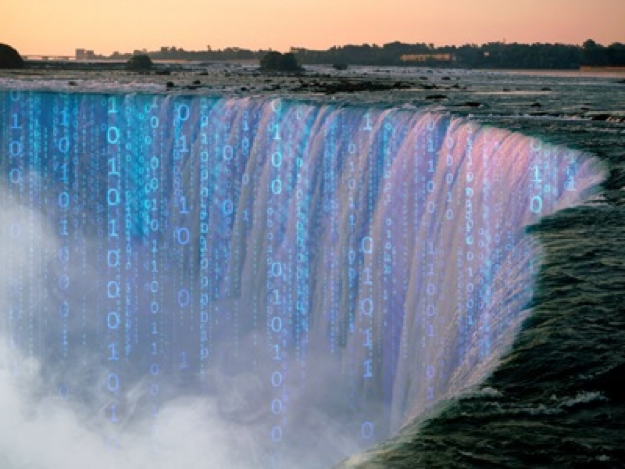
\includegraphics[width=1.0\textwidth]{bigdata}
		\end{center}
	\end{column}
\end{columns}

\begin{block}{\centering Approach}
	\begin{center}
		Use data stream and distributed memory models
	\end{center}
\end{block}

\end{frame}



%------------------------------------------------

\begin{frame}
\frametitle{Centrality Indices}


\begin{columns}
\begin{column}{0.6\textwidth}
	\begin{itemize}
		\item Assign scores to vertices or edges
		\begin{itemize}
			\item Higher score $\rightarrow$ more important
			\item Depends on graph structure
			\item Different indices in different domains
		\end{itemize}
		\item Scores are not informative
		\begin{itemize}
			\item Usually want top $k$ elements
		\end{itemize}
		\item Relative order-preserving approximation is acceptable
	%	\item Data warehousing becomes difficult
	%	\begin{itemize}
	%		\item parallelization, pass-contrained computation
	%	\end{itemize}
	\end{itemize}
\end{column}
\begin{column}{0.4\textwidth}  %%<--- here
\begin{center}
	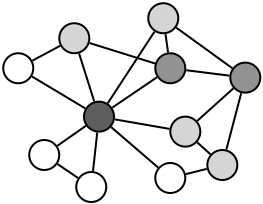
\includegraphics[width=1.0\textwidth]{centrality_greyscale}
\end{center}
\end{column}

\end{columns}

\begin{block}{}
	\begin{center}
		Exact algorithms do not scale to massive graphs
	\end{center}
\end{block}

\end{frame}

%------------------------------------------------

 \begin{frame}
\frametitle{Massive-Scale Graph Centrality}

\textbf{The Problem}
\begin{itemize}
	\item High Memory, Computation, Comunication cost
	\item Wasted effort 
	\begin{itemize}
		\item Generally only need top elements vis-\'a-vis a centrality index
	\end{itemize}
\end{itemize}
\textbf{Our Solution}
\begin{itemize}
	\item Sketch data structures
	\begin{itemize}
		\item Utilize composable streaming summaries of vertex-local information
	\end{itemize}
	\item Distributed memory
	\begin{itemize}
		\item Partition graph and distribute sketches
		\item Polyloglinear computation, memory, and communication
	\end{itemize}
\end{itemize}

\end{frame}

%------------------------------------------------

\begin{frame}
\frametitle{Overcoming Data Scale: Data Streaming}


\begin{columns}
\begin{column}{0.55\textwidth}
	\begin{itemize}
		\item Traditional RAM algorithms scale poorly
		\begin{itemize}
			\item Awkward to store data in memory
			\item Superlinear scaling unacceptable
		\end{itemize}
		\item Data stream model to the rescue!
		\begin{itemize}
			\item Sequential data access
			\item Sublinear memory
			\item Nearly linear amortized time
			\item Constrained number of passes
			\item Monte Carlo Approximations
		\end{itemize}
%		\item Increasingly want to 
%		\item \emph{Centrality} captures the ``importance'' of a vertex
%		\begin{itemize}
%			\item Many different measures
%			\item Expensive to recompute whenever graph changes
%		\end{itemize}
	%	\item Data warehousing becomes difficult
	%	\begin{itemize}
	%		\item parallelization, pass-contrained computation
	%	\end{itemize}
	\end{itemize}
\end{column}
\begin{column}{0.45\textwidth}  %%<--- here
\begin{center}
	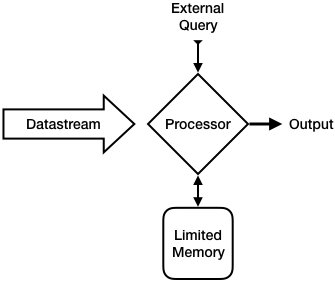
\includegraphics[width=1.0\textwidth]{stream_model}
\end{center}
\end{column}

\end{columns}
\end{frame}

%------------------------------------------------

\begin{frame}
\frametitle{Overcoming Data Scale: Distributed Data Streaming}


\begin{columns}
\begin{column}{0.6\textwidth}
	\begin{itemize}
		\item Distributed memory model a staple of HPC
		\begin{itemize}
			\item Divide computation
			\item Immense scaling
		\end{itemize}
		\item Why not distributed data streams!?!
		\begin{itemize}
			\item \textbf{Sketches} - composable summaries
			\item vertex-centric algorithms
			\item Even greater scaling
			\item Linear communication
		\end{itemize}
%		\item Increasingly want to 
%		\item \emph{Centrality} captures the ``importance'' of a vertex
%		\begin{itemize}
%			\item Many different measures
%			\item Expensive to recompute whenever graph changes
%		\end{itemize}
	%	\item Data warehousing becomes difficult
	%	\begin{itemize}
	%		\item parallelization, pass-contrained computation
	%	\end{itemize}
	\end{itemize}
\end{column}
\begin{column}{0.4\textwidth}  %%<--- here
\begin{center}
	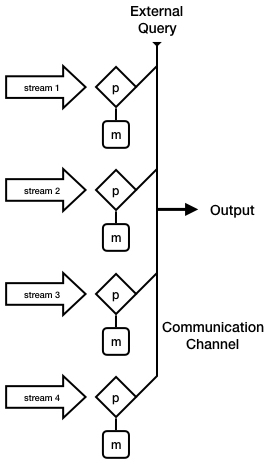
\includegraphics[width=0.9\textwidth]{dist_stream_model}
\end{center}
\end{column}

\end{columns}
\end{frame}


%\begin{frame}
%\frametitle{Important Centrality Indices}
%
%
%\begin{itemize}
%	\item $O(n)$ space
%	\begin{itemize}
%		\item Degree Centrality
%	\end{itemize}
%	\vspace{-0.0cm}
%	\begin{equation*}
%		\textnormal{DC}(x) = |\{(u,v) \in E \mid x \in \{u,v\} \}| = \|A_{x,:}\|_1 = \|A_{:,x}\|_1
%%		\textnormal{IDC}(x) &= |\{(u,v) \in E \mid x=v\}| = \|A_{x,:}\|_1 \\
%%		\textnormal{ODC}(x) &= |\{(u,v) \in E \mid x=u\}| = \|A_{:,x}\|_1
%	\end{equation*}
%	\vspace{-0.7cm}
%	\item $O(m)$ space
%	\begin{itemize}
%		\item Closeness Centrality
%		\vspace{-0.1cm}
%		\begin{equation*}
%			\textnormal{CC}(x) = \frac{1}{\sum\limits_{y \in V} d(x,y)}
%		\end{equation*}
%		\vspace{-0.7cm}
%		\item Betweenness Centrality
%		\begin{equation*}
%			\textnormal{BC}(x) = \sum\limits_{\substack{x \not\in \{y,z\} \\ \lambda_{y,z} \neq 0}} \frac{\lambda_{y,z}(x)}{\lambda_{y,z}}
%		\end{equation*}
%		\item $\kappa$-Path Centrality
%		\vspace{-0.2cm}
%		\begin{equation*}
%			\textnormal{PC}(x, \kappa) = \Pr [x \in \text{ a random simple path of length $\leq \kappa$} ]
%		\end{equation*}
%		\item Eigencentrality
%		\vspace{-0.2cm}
%		\begin{equation*}
%			\textnormal{EC}(x) = u_{x} \text{, where $u$ is the dominant left eigenvector of $A$}
%		\end{equation*}
%	\end{itemize}
%\end{itemize}
%\end{frame}

%------------------------------------------------

%----------------------------------------------------------------------------------------
%----------------------------------------------------------------------------------------
%\section{Background}
%----------------------------------------------------------------------------------------
%----------------------------------------------------------------------------------------


%\begin{frame}
%\frametitle{Graph Primitives}
%
%Assume throughout that $\mathcal{G}=(\mathcal{V}, \mathcal{E}, \mathbf{w})$, where $|\mathcal{V}| = n$ and $|\mathcal{E}| = m$
%
%\begin{itemize}
%	\item $\mathbf{w}_e$ is the weight of edge $e$ if $e \in \mathcal{E}$ and zero otherwise
%	\item $\mathcal{G}$ has adjacency matrix $A \in \mathbb{R}^{n \times n}$ so that $A_{x,y} = \textbf{w}_{xy}$ for $xy \in \mathcal{E}$
%	\item $\mathcal{G}$ has vertex-edge incidence matrix $B \in \mathbb{R}^{{n \choose 2} \times n}$ so that 
%$B_{xy,z} = 
%\begin{cases}
%\textbf{w}_{xy} & \textnormal{if $x=z$} \\
%-\textbf{w}_{xy} & \textnormal{if $y=z$} \\
%0 & \textnormal{else}.
%\end{cases}$
%\end{itemize}
%
%
%\begin{columns}
%
%\begin{column}{0.35\textwidth}
%\begin{center}
%\tikz \graph [nodes={draw,circle}] { a -- {b, c} -- d };
%\end{center}
%\end{column}
%
%\begin{column}{0.65\textwidth}
%\[
%B=
%\begin{blockarray}{ccccc}
%& a & b & c & d \\
%\begin{block}{c(cccc)}
%  ab & 1 & -1 & 0 & 0 \\
%  ac & 1 & 0 & -1 & 0 \\
%  ad & 0 & 0 & 0 & 0 \\
%  bc & 0 & 0 & 0 & 0 \\
%  bd & 0 & 1 & 0 & -1 \\  
%  cd & 0 & 0 & 1 & -1 \\
%\end{block}
%\end{blockarray}
% \]
%\end{column}
%\end{columns}
%
%\end{frame}

%------------------------------------------------

\begin{frame}
\frametitle{Streaming Background}

Assume throughout that $\mathcal{G}=(\mathcal{V}, \mathcal{E}, \mathbf{w})$, where $|\mathcal{V}| = n$ and $|\mathcal{E}| = m$

\begin{itemize}
	\item $\mathbf{w}_e$ is the weight of edge $e$ if $e \in \mathcal{E}$ and zero otherwise
	\item $\mathcal{G}$ has adjacency matrix $A \in \mathbb{R}^{n \times n}$ so that $A_{x,y} = \textbf{w}_{xy}$ for $xy \in \mathcal{E}$
\end{itemize}

$\mathcal{G}$ is given by a \emph{stream} $\sigma$
\begin{itemize}
	\item A list of edge insertions (\emph{insert-only})
	\item If deletions exist, say \emph{turnstile stream}
\end{itemize}

An algorithm accumulating a data structure $\mathcal{S}$ and is called...
\begin{itemize}
	\item \emph{streaming} if $\mathcal{S}$ uses $\widetilde{O}(1) = O(\log n)$
	\footnote{\scriptsize $\widetilde{O}()$ notation suppresses polylogarithmic factors} memory
	\item \emph{semi-streaming} if $\mathcal{S}$ uses $\widetilde{O}(n) = O(n \polylog n)$
	\footnote{\scriptsize sometimes $\widetilde{O} \left (n^{1+\alpha} \right )$ for $\alpha \in (0,1/2]$} memory
\end{itemize}

Want to minimize the number of passes over $\sigma$	
\begin{itemize}
	\item 1 pass ideal
	\item Constant or logarithmic passes sometimes acceptable 
\end{itemize}

\end{frame}

%------------------------------------------------

%\begin{frame}
%\frametitle{Streaming Background}
%
%\begin{itemize}
%	\item A \emph{stream} $\sigma$ accumulating $\mathbf{f} \in \mathbb{R}^{n}$ is a list of index updates
%	\begin{itemize}
%		\item An update $(i,c)$ means $\mathbf{f} \gets \mathbf{f} + c*e_i$
%		\item A \emph{cash register} stream enforces $c > 0$ for all updates
%		\item A \emph{turnstile} stream allows negative updates
%		\item A \emph{strict turnstile} stream allows negatives but enforces $\mathbf{f} \in \mathbb{R}^{n}_{\geq 0}$
%	\end{itemize}
%	\item An algorithm accumulating a data structure $\mathcal{S}$ and is said to be...
%	\begin{itemize}
%		\item \emph{streaming} if $\mathcal{S}$ uses $\widetilde{O}(1) = O(\log n)$
%		\footnote{\scriptsize $\widetilde{O}()$ notation suppresses polylogarithmic factors} memory
%		\item \emph{semi-streaming} if $\mathcal{S}$ uses $\widetilde{O}(n) = O(n \polylog n)$
%		\footnote{\scriptsize sometimes $\widetilde{O} \left (n^{1+\alpha} \right )$ for $\alpha \in (0,1/2]$} memory
%	\end{itemize}
%	\item Want to minimize the number of passes over $\sigma$	
%	\begin{itemize}
%		\item 1 pass ideal
%		\item Constant or logarithmic passes sometimes acceptable 
%	\end{itemize}
%
%\end{itemize}
%
%\end{frame}

%------------------------------------------------

\begin{frame}
\frametitle{Sketching}

\begin{definition}[Sketch]
A \emph{Sketch} is a streaming data structure $\mathcal{S}$ that admits a merge operator $\oplus$. 
If $\circ$ is the stream concatenation operator, then for any streams $\sigma_1$ and $\sigma_2$,
\begin{equation*}
	\mathcal{S}(\sigma_1) \oplus \mathcal{S}(\sigma_2) = \mathcal{S}(\sigma_1 \circ \sigma_2).
\end{equation*}
\end{definition}

\begin{definition}[Linear Sketch]
A \emph{Linear Sketch} $\mathcal{S}$ is a linear projection of $\mathbf{f}$ to a lower dimension.
For any streaming frequency vectors $\mathbf{f}_1$ and $\mathbf{f}_2$ and scalars $a$ and $b$, 
\begin{equation*}
	a\mathcal{S}(\mathbf{f}_1) + b\mathcal{S}(\mathbf{f}_2) = \mathcal{S}(a\mathbf{f}_1 + b\mathbf{f}_2).
\end{equation*}
\end{definition}

\begin{block}{}
\begin{center}
%	\vspace{-1.1em}
	Sketches are useful for stream summarization when \\
	\emph{comparisons between streams} are important
\end{center}
\end{block}

\end{frame}

%------------------------------------------------

\begin{frame}
\frametitle{Proposal Refresh}

\begin{enumerate}
	\item Semi-streaming approximation of betweenness centrality heavy hitters
	\begin{itemize}
		\item Semi-streaming simulation of $k$ random walks of length $t$
		\begin{itemize} 
			\item Lower and almost-tight upper bound algorithm
		\end{itemize}
		\item Semi-streaming $\kappa$-path centrality algorithm
	\end{itemize}
	\item Semi-streaming eigencentrality approximation 
	\begin{itemize}
		\item Explored at length by Eisha R. Nathan in \cite{nathan2018numerical}
		\begin{itemize}
			\item Mostly applied to Katz's Index
		\end{itemize}
	\end{itemize}
	\item Sketch robustness analysis 
	\begin{itemize}
		\item Analysis of HyperLogLog cardinality sketches and their intersections
	\end{itemize}
	\item Implementation and empirical evaluation of semi-streaming graph algorithms 
	\begin{itemize}
		\item Implementation of \algoname{YGM} communication protocol
%		\begin{itemize}
%			\item Powers HPC algorithms with asymmetric computational loads
%		\end{itemize}
		\item Implementation of \algoname{DegreeSketch} and related algorithms
		\begin{itemize}
			\item Local neighborhood size and triangle count 
		\end{itemize}
	\end{itemize}
\end{enumerate}


\end{frame}

%------------------------------------------------
%------------------------------------------------
\section{Summary of Results}
%------------------------------------------------
%------------------------------------------------

\againframe<3>{overview}

\begin{frame}
\frametitle{Summary of Results: Serial Algorithms}

%Degree centrality
\begin{dynblock}
% First block
\opaqueblock<1->{
Degree Centrality
%
\vspace{-0.2cm}
%
\begin{equation*}
	\mathcal{C}^{\algoname{Deg}}(x) = |\{(u,v) \in E \mid x \in \{u,v\} \}| = \|A_{x,:}\|_1 = \|A_{:,x}\|_1
\end{equation*}
%
\vspace{-0.8cm}
%
\begin{itemize}
	\item Na\"ive online $O(n)$-space and -time algorithm exists
\end{itemize}
}

\invblock<2->

% Second block
\opaqueblock<2->[0.8\textwidth]{
\begin{center}
	\vspace{-1.1em}
	We show $\widetilde{O}(1)$-space distributable streaming algorithms
\end{center}
}
\end{dynblock}



%close/between centrality
\begin{dynblock}
% First block
\opaqueblock<3>{
Closeness Centrality
%
\vspace{-0.2cm}
%
\begin{equation*}
	\mathcal{C}^{\algoname{Close}}(x) = \frac{1}{\sum\limits_{y \in V} d(x,y)}
\end{equation*}
%
\vspace{-0.4cm}
%
\begin{itemize}	
	\item Online exact $O(n^2)$-space $O(nm)$-time algorithm \cite{wei2014real}
	\item Batch Approximate $O(n^2)$-space and almost-linear time algorithm \cite{cohen2014computing}
\end{itemize}
}

\invblock<4->

% Second block
\opaqueblock<4->[0.75\textwidth]{
\begin{center}
	\vspace{-1.1em}
	We show constant-pass semi-streaming algorithm
\end{center}
}

\end{dynblock}

\end{frame}

%------------------------------------------------

\begin{frame}
\frametitle{Summary of Results: Distributed Streaming Algorithms}

%Degree centrality
\begin{dynblock}
% First block
\opaqueblock<1->{
Local $t$th Neighborhood Centrality
%
\vspace{-0.2cm}
%
\begin{align*}
	\mathcal{N}(t)  
	&= |\{(x, y) \in \mathcal{V} \times \mathcal{V} | d_\mathcal{G}(x, y) < t\}| 
	& \textnormal{(global) $t$th neighborhood} \\
	\mathcal{C}^{\algoname{Nbhd}}_t(x)  
	&= |\{y \in \mathcal{V} | d_\mathcal{G}(x, y) < t\}|
	& \textnormal{(local) $t$th neighborhood} \\	
\end{align*}
%
\vspace{-1.3cm}
%
\begin{itemize}
	\item Serial estimation algorithms ANF \cite{palmer2002anf} and HyperANF \cite{boldi2011hyperanf}
\end{itemize}
}


%\invblock<2->
%
%% Second block
%\opaqueblock<2->[0.8\textwidth]{
%\begin{center}
%	\vspace{-1.1em}
%	We show $\widetilde{O}(\varepsilon^{-2}n)$-space distributable streaming algorithms
%\end{center}
%}
\end{dynblock}


%close/between centrality
\begin{dynblock}
% First block
\opaqueblock<1->{
	\begin{center}
		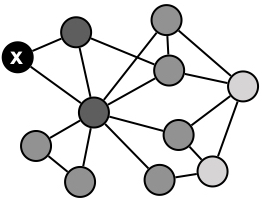
\includegraphics[width=0.35\textwidth]{nbhd_fig_landscape}
	\end{center}
%\vspace{-1.1em}
%We demonstrate a $t$-pass, semi-streaming, distributed \algoname{DegreeSketch}-based algorithm for estimating $\mathcal{N}(t)$ and $\mathcal{C}^{\algoname{Nb}}_t(x)$ for each $x \in \mathcal{V}$
%\cite{priest2019degreesketch}.
%%[PPS18, PPS19]
%%\footnote{\tiny Benjamin W. Priest, Roger Pearce and Geoffrey Sanders, ``Estimating Edge-Local Triangle Count Heavy Hitters in Edge-Linear Time and Almost-Vertex-Linear Space,'' HPEC 2018}
%\footnote{\tiny Benjamin W. Priest, Roger Pearce and Geoffrey Sanders, ``\algoname{DegreeSketch}: Distributed Cardinality Sketches on Graphs, with Applications,'' In preparation for SigKDD 2019}
}

\invblock<2->

% Second block
\opaqueblock<2->{
We demonstrate a $t$-pass, semi-streaming, distributed \algoname{DegreeSketch}-based algorithm for estimating $\mathcal{N}(t)$ and $\mathcal{C}^{\algoname{Nbhd}}_t(x)$ for each $x \in \mathcal{V}$
\cite{priest2019degreesketch}.
%[PPS18, PPS19]
%\footnote{\tiny Benjamin W. Priest, Roger Pearce and Geoffrey Sanders, ``Estimating Edge-Local Triangle Count Heavy Hitters in Edge-Linear Time and Almost-Vertex-Linear Space,'' HPEC 2018}
\footnote{\tiny Benjamin W. Priest, Roger Pearce and Geoffrey Sanders, ``\algoname{DegreeSketch}: Distributed Cardinality Sketches on Graphs, with Applications,'' In preparation for SigKDD 2019}
}


\end{dynblock}



\end{frame}




%------------------------------------------------

\begin{frame}
\frametitle{Summary of Results: Distributed Streaming Algorithms}

%Degree centrality
\begin{dynblock}
% First block
\opaqueblock<1->{
Triangle Count Centrality
%
\vspace{-0.2cm}
%
\begin{align*}
	\mathcal{C}^{\algoname{Tri}}(x) 
	&= |\{yz \in \mathcal{E} \mid xy, yz, xz \in \mathcal{E} \}| 
	& \textnormal{(vertex-local)} \\
	\mathcal{C}^{\algoname{Tri}}(xy) 
	&= |\{z \in \mathcal{E} \mid xy, yz, xz \in \mathcal{E} \}|
	& \textnormal{(edge-local)} \\	
\end{align*}
%
\vspace{-1.3cm}
%
\begin{itemize}
	\item Exact $O(m)$-space, $O \left ( m^{\frac{3}{2}} \right )$-time serial and distributed algorithms \cite{arifuzzaman2013patric, pearce2017triangle}
	\footnote{\tiny Roger Pearce, ``Triangle counting for scale-free graphs at scale in distributed memory,'' HPEC 2017}
	\item Semi-streaming sampling algorithms \cite{lim2015mascot, stefani2017triest} and distributed generalizations \cite{shin2018tri, shin2018dislr}
%	\begin{itemize}
%		\item Including distributed generalizations 
%	\end{itemize}
\end{itemize}
}
\end{dynblock}


%close/between centrality
\begin{dynblock}
\opaqueblock<1->{
	\begin{columns}
	\begin{column}{0.3\textwidth}
		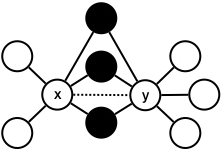
\includegraphics[width=1.0\textwidth]{edge_local}
	\end{column}
	\begin{column}{0.3\textwidth}
		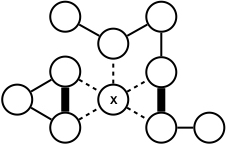
\includegraphics[width=1.0\textwidth]{vertex_local}
	\end{column}
	\end{columns}
}

\invblock<2->

\opaqueblock<2>{
We show 2-pass, semi-streaming, distributed \algoname{DegreeSketch}-based algorithms for estimating heavy hitters 
\cite{priest2018estimating, priest2019degreesketch}
\footnote{\tiny Benjamin W. Priest, Roger Pearce and Geoffrey Sanders, ``Estimating Edge-Local Triangle Count Heavy Hitters in Edge-Linear Time and Almost-Vertex-Linear Space,'' HPEC 2018}
\footnote{\tiny Benjamin W. Priest, Roger Pearce and Geoffrey Sanders, ``\algoname{DegreeSketch}: Distributed Cardinality Sketches on Graphs, with Applications,'' In preparation for SigKDD 2019}
}

\end{dynblock}



\end{frame}




%------------------------------------------------



\begin{frame}
\frametitle{Summary of Results: Distributed Streaming Algorithms}

%Degree centrality
\begin{dynblock}
% First block
\opaqueblock<1->{
Semi-streaming simulation of $k$ random walks of length $t$
%
%\vspace{-0.2cm}
%
%\begin{equation*}
%	\mathcal{C}^{\algoname{$\kappa$}}(x)  =  \Pr_{p: |p| \leq \kappa} [x \in p \wedge \text{$p$ a simple path } ]
%\end{equation*}
%
%\vspace{-0.6cm}
%
\begin{itemize}	
	\item $O(nkt)$-space trivial algorithm
	\item $\Omega \left ( n\sqrt{t} \right )$ lower bound and almost-tight upper bound for simulating a single random walk of length $t$ \cite{jin2018simulating}.
%	\begin{itemize}
%		\item Online exact and approximate $O(n^2)$- and $O(m)$-space algorithms exist \cite{green2012fast, wei2014real, kourtellis2015scalable, bergamini2014approximating}%, [GMB12], [WC14], [KMB15], [BMS15]
%	\end{itemize}
\end{itemize}
}
\end{dynblock}


%close/between centrality
\begin{dynblock}
% First block
\opaqueblock<2>{
\begin{itemize}
	\item	We show $\Omega \left ( n\sqrt{kt} \right )$ space lower bound
	\item	We demonstrate an $O \left ( n\sqrt{kt}\frac{\log q}{q} \right )$ algorithm with failure probability $\varepsilon$, where $q = 2 + \frac{\log (1/\varepsilon)}{\sqrt{kt}}$ on insert-only streams.
	\item We demonstrate a distributed version of this algorithm, and describe how to generalize it to a faultless system utilizing the \emph{playback} of adjacency substreams.
\end{itemize}
}

\end{dynblock}

\end{frame}



%------------------------------------------------



\begin{frame}
\frametitle{Summary of Results: Distributed Streaming Algorithms}

%Degree centrality
\begin{dynblock}
% First block
\opaqueblock<1->{
$\kappa$-Path Centrality
%
\vspace{-0.2cm}
%
\begin{equation*}
	\mathcal{C}^{\algoname{Path}}_{\kappa}(x)  =  \Pr_{p: |p| \leq \kappa} [x \in p \wedge \text{$p$ a simple path } ]
\end{equation*}
%
\vspace{-0.6cm}
%
\begin{itemize}	
	\item $O(m)$-space $O(n^{1 + \alpha} \log^{2} n)$-time approximation algorithm \cite{kourtellis2013identifying}
	\item Empirical proxy for betweenness centrality heavy hitters
	\begin{itemize}
		\item Online exact and approximate $O(n^2)$- and $O(m)$-space algorithms exist \cite{green2012fast, wei2014real, kourtellis2015scalable, bergamini2014approximating}%, [GMB12], [WC14], [KMB15], [BMS15]
	\end{itemize}
\end{itemize}
}
\end{dynblock}


%close/between centrality
\begin{dynblock}
% First block
\opaqueblock<2>{
\begin{itemize}
	\item	We show how to use the distributed random walk simulation framework with playback to estimate $\kappa$-path centrality at scale
	\item	Yields sublinear distributed $\kappa$-path centrality approximation algorithm
\end{itemize}
}

\end{dynblock}







\end{frame}



%------------------------------------------------



\begin{frame}
\frametitle{Summary of Results}

%Degree centrality


\begin{table}[htbp]
\caption{Summary of Algorithmic Results \label{tab:scaling_graphs}}
\begin{center}
\resizebox{\textwidth}{!}{
\begin{tabular}{|c|c|c|c|c|c|c|}
\hline
\textbf{Problem} & passes & distributed? & dynamic? &  analytic bound? & lower bound? & experiments? \\
\hline
\hline
Degree Centrality & 1 & & \checkmark & \checkmark &  & \\
\hline
Closeness Centrality & O(1) & & \checkmark & \checkmark & & \\
\hline
$t$th Neighborhood & $t$ & \checkmark & & \checkmark & & \\
\hline
Local Triangle Counts & 2 & \checkmark & &  & & \checkmark \\
\hline
$k$ $t$-step Random Walks & 1\footnote{Changes when subject to playback} & \checkmark& \checkmark & \checkmark & \checkmark & \\
\hline
$\kappa$-Path Centrality & $*$ & \checkmark& \checkmark & \checkmark & & \\
\hline
\end{tabular}
}
\end{center}
\end{table}





\end{frame}



%------------------------------------------------

%\begin{frame}
%\frametitle{Some Important Sketches}
%
%\begin{dynblock}
%% Tug-of-War
%\opaqueblock<1>{
%%
%\begin{tabular*}{\textwidth}{l @{\extracolsep{\fill}} r}
%\algoname{Tug-of-War} & \cite{alon1999space}%[AMS99]
%\end{tabular*}
%%
%\vspace{-0.5cm}
%%
%\begin{itemize}
%\item 4-universal hash function $h: [n] \rightarrow \{-1,1\}$
%\item Define $s \in \mathbb{R}^{n}$: $s^T = (h(1), \dots, h(n))$
%\item Accumulate $s^Tv$
%\end{itemize}
%}
%\invblock<2->
%
%% Second block
%\opaqueblock<2->[0.6\textwidth]{
%%
%\vspace{-0.5cm}
%%
%\begin{center}
%$(1\pm \varepsilon)$-approx of $F_2(v)$ w.h.p.
%\end{center}
%}
%%\invblock<5->
%%
%% Third block
%%\opaqueblock<5>[0.5\textwidth]{
%%%
%%\vspace{-0.3cm}
%%%
%%\begin{center}
%% $O \left ( \frac{\log(1/\delta)}{\varepsilon^{2}} (\log n + \log m) \right )$ space
%%\end{center}
%%}
%
%\end{dynblock}
%
%
%\begin{dynblock}
%% CountSketch
%\opaqueblock<3>{
%%
%\begin{tabular*}{\textwidth}{l @{\extracolsep{\fill}} r}
%\algoname{CountSketch} & \cite{charikar2002finding}%[CCFC04]
%\end{tabular*}
%%
%\vspace{-0.5cm}
%%
%\begin{itemize}
%\item 2-universal hash functions $h: [n] \rightarrow [r]$ and $s: [n] \rightarrow \{-1,1\}$
%\item Define $C \in \mathbb{R}^{r \times n}$: $C = \{0\}^{r \times n}$, $\forall j \in [n]$, $C_{h(j),j} = s(j)$
%\item Accumulate $Cv$
%\end{itemize}
%}
%%\invblock<2->
%\invblock<4->
%
%% Second block
%\opaqueblock<4->[0.7\textwidth]{
%Produce $\tilde{f}$ s.t. $\forall j \in [n]$, $|\tilde{f}(j) - v_j | \leq \varepsilon \|v_{-j}\|_2$ w.h.p.
%}
%%\invblock<5->
%%
%%% Third block
%%\opaqueblock<5>[0.3\textwidth]{
%%%
%%\vspace{-0.3cm}
%%%
%%\begin{center}
%%$O \left ( \frac{\log(n/\delta)}{\varepsilon^{2}} \right )$ space
%%\end{center}
%%}
%
%\end{dynblock}
%
%
%
%
%\begin{dynblock}
%% JLT
%\opaqueblock<5>{
%%
%\begin{tabular*}{\textwidth}{l @{\extracolsep{\fill}} r}
%Johnson-Lindenstrauss Transform (Gaussian variant) & \cite{har2012approximate} %[IM98]
%\end{tabular*}
%%
%\vspace{-0.5cm}
%%
%\begin{itemize}
%\item $R \in \mathbb{R}^{r \times n}$, where $R_i,j \sim \mathcal{N}(0,1)$ $\forall i,j$
%\item $S = \frac{1}{\sqrt{r}} R$
%\item Accumulate $Sv$
%\end{itemize}
%}
%%\invblock<2->
%\invblock<6->
%
%% Second block
%\opaqueblock<6>[0.6\textwidth]{
%$\forall v, v^\prime \in \mathbb{R}^n$:
%%
%\vspace{-0.3cm}
%%
%\begin{center}
%$\langle Sv, Sv^\prime \rangle - \langle v, v^\prime \rangle \leq \varepsilon \|v\|_2 \|v^\prime\|_2$ w.h.p.
%\end{center}
%}
%%\invblock<5->
%%
%%% Third block
%%\opaqueblock<5>[0.3\textwidth]{
%%%
%%\vspace{-0.3cm}
%%%
%%\begin{center}
%%$O \left ( \frac{\log(n/\delta)}{\varepsilon^{2}} \right )$ space
%%\end{center}
%%}
%
%\end{dynblock}
%
%
%
%\end{frame}

%------------------------------------------------



%\begin{frame}
%\frametitle{Important Applications}
%
%\begin{dynblock}
%% l2 sampling
%\opaqueblock<1>{
%%
%\begin{tabular*}{\textwidth}{l @{\extracolsep{\fill}} r}
%$\ell_p$-sampling & \cite{monemizadeh20101,jowhari2011tight}%[MW10], [JST11]
%\end{tabular*}
%%
%\vspace{-0.5cm}
%%
%\begin{itemize}
%\item Sample $t_i \sim_R (0,1)$ $\forall i \in [n]$
%\item Rescale updates to $v_i$ by $1/t_i^{1/p}$
%\item Accumulate \algoname{Tug-of-War}, \algoname{CountSketch}, and $\ell_p$-norm sketches
%\item Use sketches to output \algoname{CountSketch} argmax or FAIL
%\end{itemize}
%}
%\invblock<2->
%
%% Second block
%\opaqueblock<2->[0.6\textwidth]{
%%
%\vspace{-0.5cm}
%%
%\begin{center}
%Outputs $(i,P)$ w.h.p., where $i \in [n]$ is sampled w.p. $P = (1 \pm \varepsilon)\frac{|v_i|^p}{\|v\|^p_p}$ 
%\end{center}
%}
%%\invblock<3->
%%
%%% Second block
%%\opaqueblock<3->[0.7\textwidth]{
%%%
%%\vspace{-0.5cm}
%%%
%%\begin{center}
%%$O(\log^2n \log (1/\delta))$ space for $p=0$ \\
%%$O(\varepsilon^{-1}\log(1/\varepsilon)\log^2n \log (1/\delta))$ space for $p=1$ \\
%%\end{center}
%%}
%
%\end{dynblock}
%
%
%
%\begin{dynblock}
%% rank-k approximation
%\opaqueblock<3>{
%%
%\begin{tabular*}{\textwidth}{l @{\extracolsep{\fill}} r}
%Rank-$k$ Approximation (1-pass) & \cite{clarkson2009numerical}%[CW09]
%\end{tabular*}
%%
%\vspace{-0.5cm}
%%
%\begin{itemize}
%\item Given $A \in \mathbb{R}^{n \times d}$
%\item Sample JLTs $S \in \mathbb{R}^{(r/\varepsilon^2) \times n}$, $R \in \mathbb{R}^{d \times r}$
%\item Accumulate $SA$, $AR$, $SAR$
%\item Compute $U$, an orthonormal basis for the rowspace of $AR$
%\item Return $U[U^TAR(SAR)^+SA]_k$
%\end{itemize}
%}
%\invblock<4->
%
%% Second block
%\opaqueblock<4>[0.6\textwidth]{
%%
%\vspace{-0.5cm}
%%
%\begin{center}
%Outputs rank-$k$ factored $\tilde{A}_k$ s.t. $\|A - \tilde{A}_k \|_F \leq (1 + \varepsilon) \|A - A_k\|_F$ w.h.p.
%\end{center}
%}
%%\invblock<6>
%%
%%% Second block
%%\opaqueblock<6>[0.5\textwidth]{
%%%
%%\vspace{-0.5cm}
%%%
%%\begin{center}
%%$O(k\varepsilon^{-2}(n + d\varepsilon^{-2})\log (nd/\delta))$ space
%%\end{center}
%%}
%
%\end{dynblock}
%
%
%
%
%\end{frame}


%----------------------------------------------------------------------------------------
%----------------------------------------------------------------------------------------
%\section{Serial Streaming Algorithms}
%----------------------------------------------------------------------------------------
%----------------------------------------------------------------------------------------






%\begin{frame}
%\frametitle{Degree Centrality}
%
%\begin{columns}
%\begin{column}{0.5\textwidth}
%	\begin{itemize}
%		\item The degree centrality of a vertex is its valency
%		\item High degree-central vertices have many connections
%		\item Let $v \in \mathbb{R}^n$ be the vector of degree centralities
%		\begin{itemize}
%			\item $v_x$ is the row sum of $A_{x,:}$
%			\item $\sigma$ updating $A$ implicitly updates $v$
%		\end{itemize}
%	%	\item Data warehousing becomes difficult
%	%	\begin{itemize}
%	%		\item parallelization, pass-contrained computation
%	%	\end{itemize}
%	\end{itemize}
%\end{column}
%\begin{column}{0.5\textwidth}  %%<--- here
%\begin{center}
%	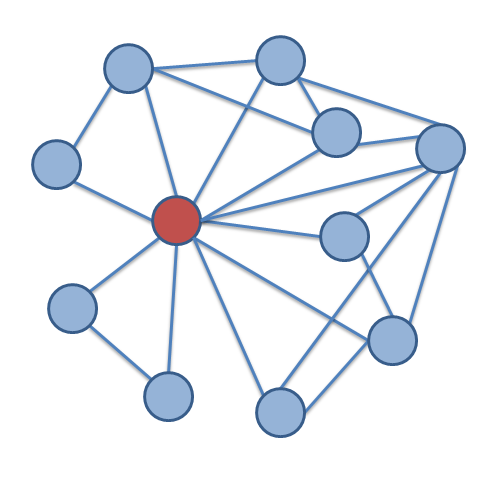
\includegraphics[width=1.0\textwidth]{centrality}
%\end{center}
%\end{column}
%
%\end{columns}
%\end{frame}

%------------------------------------------------

%\begin{frame}
%\frametitle{\algoname{CountSketch}}
%
%\begin{columns}
%\begin{column}{0.65\textwidth}
%	\begin{itemize}
%		\item Consider 2-universal hash functions
%		\begin{itemize}
%			\item $h_1, \dots, h_t : [n] \rightarrow [r]$
%			\item $s_1, \dots, s_t : [n] \rightarrow \{-1,1\}$
%		\end{itemize}
%		\item Define $C^{(i)} \in \mathbb{R}^{r \times n}$:
%		\begin{itemize}
%			\item $C^{(i)}_{h(j),j} \gets s(j)$ for each $j \in [n]$
%		\end{itemize}
%		\item $(C^{(i)}v)_x*s(x)$ is a good estimator for $v_x$
%		\item $\med_{i \in [t]} \{(C^{(i)}v)_x*s_i(x) \}$ has low variance
%	%	\item Data warehousing becomes difficult
%	%	\begin{itemize}
%	%		\item parallelization, pass-contrained computation
%	%	\end{itemize}
%	\end{itemize}
%\end{column}
%\begin{column}{0.35\textwidth}  %%<--- here
%\begin{center}
%	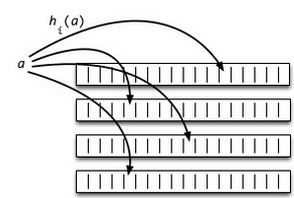
\includegraphics[width=1.0\textwidth]{CS}
%\end{center}
%\end{column}
%
%\end{columns}
%
%
%\begin{theorem}[\algoname{CountSketch}]
%%Let $v \in \mathbb{R}^n$ and $C_1, \dots, C_t \in \mathbb{R}^{r \times n}$ be \algoname{CountSketch} matrices.
%For every $j \in n$ let $\tilde{v}_j = \med_{i \in [t]} \{(C^{(i)}v)_{h(j)} * s_i(j)\}$.
%If $r= O(\varepsilon^{-2})$ and $t=O(\log(1/\delta))$, then for all $j \in [n]$ with probability at least $1-\delta$:
%%
%\begin{equation*}
%|\tilde{v}_j - v_j | \leq \varepsilon \|v_{-j}\|_2
%\end{equation*}
%%
%
%\end{theorem}
%
%\end{frame}

%------------------------------------------------

%\begin{frame}
%\frametitle{Approximating the Top $k$ Degree Centralities}
%
%\begin{definition}[\algoname{FindApproxTop}$(\sigma, k, \varepsilon)$]
%Given $\sigma$ updating $v \in \mathbb{R}^n$, $k < n$, and $\varepsilon \in \mathbb{R}^+$, output a list of $k$ indices of $v$ so that for each such index $j \in [n]$, $v_j > (1-\varepsilon)v_\ell$, where $v_\ell$ is the $k$th-largest index of $v$.
%\end{definition}
%
%\begin{itemize}
%	\item \cite{charikar2002finding} gives an algorithm using \algoname{CountSketch} that solves \algoname{FindApproxTop}$(\sigma, k, \varepsilon)$ by maintaining a heap while accumulating $C$
%	\begin{itemize}
%		\item Uses space $O \left (k \log \frac{n}{\delta} + \frac{\sum_{q = k+1}^n n_q^2}{n_k^2} \varepsilon^{-2} \log \frac{n}{\delta} \right )$ \footnote{$n_q$ is the value of the $q$th largest index of $v$}
%	\end{itemize}
%	\item Immediately applicable to degree centrality
%	\item $O((k + \varepsilon^{-2})\log (n/\delta))$ memory for strongly non-regular graphs
%\end{itemize}
%
%\end{frame}

%------------------------------------------------


%------------------------------------------------

%------------------------------------------------
%\section{Multi-Pass Semi-Streaming Closeness Centrality}
%------------------------------------------------

%------------------------------------------------

%\begin{frame}
%\frametitle{Closeness Centrality}
%
%\begin{columns}
%\begin{column}{0.6\textwidth}
%	\begin{itemize}
%		\item For vertex $x$, $CC(x) = \frac{1}{\sum_{y \in V} d(x,y)}$
%		\item High closeness-central vertices have short paths to the rest of the graph
%		\item Solving exactly requires solving \algoname{All Pairs Shortest Paths}
%		\item We solve approximately using a graph spanner obtained via $\ell_1$-sparsification on $B$, $G$'s node-edge incidence matrix
%	%	\item Data warehousing becomes difficult
%	%	\begin{itemize}
%	%		\item parallelization, pass-contrained computation
%	%	\end{itemize}
%	\end{itemize}
%\end{column}
%\begin{column}{0.4\textwidth}  %%<--- here
%\begin{center}
%	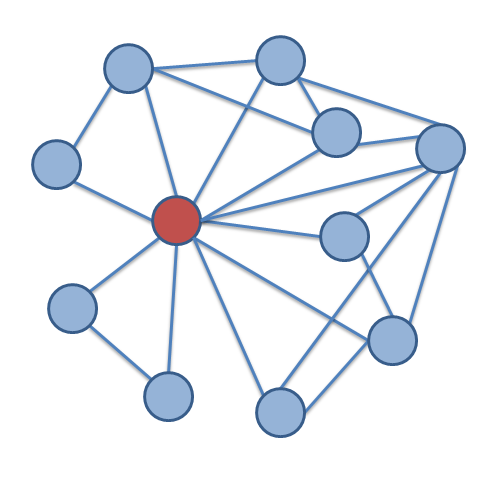
\includegraphics[width=1.0\textwidth]{centrality}
%\end{center}
%\end{column}
%
%\end{columns}
%\end{frame}

%------------------------------------------------

%----------------------------------------------------------------------------------------
%----------------------------------------------------------------------------------------
%\section{Semi-Streaming Closeness Centrality}
%----------------------------------------------------------------------------------------
%----------------------------------------------------------------------------------------




%\begin{frame}
%\frametitle{Closeness Centrality Approximation}
%
%
%\begin{definition}[$\alpha$-Spanner]
%A subgraph $H$ of $G$ such that $d_H(x,y) \leq \alpha d_G(x,y)$ for every $x,y \in V$
%\end{definition}
%
%\begin{itemize}
%	\item A sampling algorithm produces a graph spanner \cite{ahn2012graph}:
%	\begin{itemize}
%		\item Produces a $(k^{\log_2 5} - 1)$-spanner
%		\item Requires $O(n^{1+1/k})$ space
%		\item Requires $\log k$ passes
%	\end{itemize}
%	\item Trades off estimation accuracy for reduced space and passes
%	\item Can compute closeness centrality on $H$!
%\end{itemize}
%
%\end{frame}

%------------------------------------------------


%\begin{frame}
%\frametitle{Closeness Centrality Approximation, continued}
%
%
%\begin{itemize}
%	\item If $H$ is an $\alpha$-spanner of $G$, then
%{\footnotesize
%\begin{align*}
%CC_H(x) 
%= \frac{1}{\sum\limits_{y \in V} d_H(x,y)}
%\geq \frac{1}{\sum\limits_{y \in V} \alpha d_G(x,y)}
%= \frac{1}{\alpha}CC_G(x)
%\end{align*}
%}
%	\item Thus, $CC_H(x) \in \left [\frac{1}{\alpha}, 1 \right ] CC_G(x)$
%	\item \algoname{AllPairsShortestPaths} more efficient on $H$ than $G$
%	\begin{itemize}
%		\item Especially if $G$ is dense
%	\end{itemize}
%	\item Some weaknesses
%	\begin{itemize}
%		\item $\tilde{O}(n^{1+1/k})$ rather than $O(n \polylog n)$ space
%		\item No top-$k$ preservation guarantees
%		\item Greatest improvement when $G$ is dense
%		\item Not suitable for online applications
%	\end{itemize}
%\end{itemize}
%
%\end{frame}

%------------------------------------------------







%------------------------------------------------

%------------------------------------------------
%\section{Discussion of Betweenness Centrality}
%------------------------------------------------

%------------------------------------------------

%\begin{frame}
%\frametitle{Betweenness Centrality}
%
%\begin{columns}
%\begin{column}{0.7\textwidth}
%	\begin{itemize}
%		\item For $x,y,z \in V$, let $\lambda_{y,z}$ and $\lambda_{y,z}(x)$ be the number of shortest paths from $y$ to $z$ and the number which pass through $x$, respectively
%		\item For vertex $x$, $BC(x) = \sum\limits_{\substack{x \not\in \{y,z\} \\ \lambda_{y,z} \neq 0}} \frac{\lambda_{y,z}}{\lambda_{y,z}(x)}$
%		\item High betweenness-central vertices connect groups of vertices to others
%		\item Solving exactly requires solving \algoname{All Pairs All Shortest Paths}
%		\begin{itemize}
%			\item Strictly more difficult than \algoname{All Pairs Shortest Paths}
%			\item Spanner-based approach will not work
%		\end{itemize}
%		\item Many algorithms solve or approximate BC in evolving graphs, but none use sublinear memory
%	%	\item Data warehousing becomes difficult
%	%	\begin{itemize}
%	%		\item parallelization, pass-contrained computation
%	%	\end{itemize}
%	\end{itemize}
%\end{column}
%\begin{column}{0.3\textwidth}  %%<--- here
%\begin{center}
%	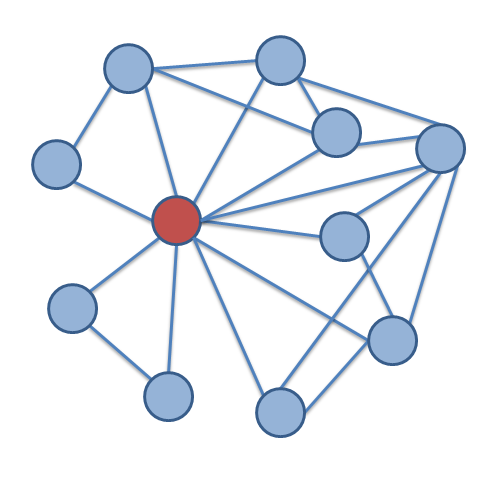
\includegraphics[width=1.0\textwidth]{centrality}
%\end{center}
%\end{column}
%
%\end{columns}
%\end{frame}
%
%%------------------------------------------------
%
%\begin{frame}
%\frametitle{A Proxy: $\kappa$-path centrality}
%
%
%\begin{definition}[$\kappa$-Path Centrality]
%For $x \in V$, $PC_\kappa(x)$ is the sum of probabilities over all $y \in V \setminus \{x\}$ that a random simple path originating at $y$ passes through $x$. 
%\end{definition}
%
%\begin{itemize}
%	\item $PC_\kappa(x)$ has been shown to correlate with $BC(x)$ in real networks for $x$ with relatively high $BC(x)$
%	\begin{itemize}
%		\item No absolute error guarantees
%	\end{itemize}
%	\item Existing approximation algorithms $\kappa$-path centrality assume a static graph
%	\item May be approximable using $\ell_1$-graph sparsification techniques
%\end{itemize}
%
%\begin{block}{}
%This approach warrants further study
%\end{block}
%
%\end{frame}

%------------------------------------------------







%------------------------------------------------

%------------------------------------------------
%\section{Spectral Centrality and A Semi-Streaming \algoname{HITS} approximation}
%------------------------------------------------

%------------------------------------------------

%\begin{frame}
%\frametitle{Spectral Measures of Centrality}
%
%\begin{itemize}
%	\item We will call any centrality measure that relies on the eigenvalues or eigenvectors of a matrix derived from $G$ \emph{spectral}
%	\begin{itemize}
%		\item e.g. Katz's index, PageRank, \algoname{HITS}, SALSA
%		\item Most require only dominant eigenvector
%	\end{itemize}
%	\item Sketching is useful for numerical linear algebra, though best results are on ``tall'' matrices
%	\item Many different semi-streaming low-rank approximations
%	\begin{itemize}
%		\item Produce factorizations similar to rank-$r$ SVD
%	\end{itemize}
%	\item Can learn the eigenvector of a rank-1 approximation so obtained
%	\begin{itemize}
%		\item However, no error guarantees
%		\item No simple way to maintain ``top $k$'' vertices
%	\end{itemize}
%\end{itemize}
%
%\end{frame}

%------------------------------------------------


%----------------------------------------------------------------------------------------
%----------------------------------------------------------------------------------------
%\section{Semi-Streaming Parallel HITS}
%----------------------------------------------------------------------------------------
%----------------------------------------------------------------------------------------


%\begin{frame}
%\frametitle{Approximating \algoname{HITS}}
%
%\begin{itemize}
%	\item \algoname{HITS} is a variant of eigencentrality producing two symbiotic scores
%	\begin{itemize}
%		\item authoritativeness: sites that are linked by hubby sites
%		\item hubbiness: sites that link to authoritative sites
%	\end{itemize}
%	\item Authoritativeness and Hubbiness converge to left dominant eigenvectors of $A^TA$ and $AA^T$, respectively
%	\begin{itemize}
%		\item If $A=U\Sigma V^T$ is the SVD, then $A^TA = V\Sigma^2V^T$ and $AA^T = U\Sigma^2U^T$
%	\end{itemize}
%	\item There is an algorithm for approximating the right singular vectors of a matrix \cite{anaraki2014memory}%[GPW12]
%	\begin{itemize}
%		\item Straightforward algorithm relying on JLTs
%	\end{itemize}
%\end{itemize}
%
%
%\begin{dynblock}
%% rank-k approximation
%\opaqueblock<2>{
%%
%Let $A = U \Sigma V^T$ be the $r$-truncated SVD of rank-$r$ $A \in \mathbb{R}^{n \times d}$. 
%Then w.h.p. the algorithm of [GPW12] returns $\tilde{V}$ so that
%\begin{equation*}
%\| V_{:,j} - \tilde{V}_{:,j}\|_2 \leq 
%\min 
%\left \{ 
%\sqrt{2}, 
%\frac{\varepsilon \sqrt{1+ \varepsilon}}{\sqrt{1-\varepsilon}}
%\max\limits_{i\neq j}
%\frac{\sqrt{2}\Sigma_{i,i} \Sigma_{j,j}}
%%{}
%{\min\limits_{c \in [-1,1]} \{| \Sigma_{i,i}^2 - \Sigma_{j,j}^2 (1 + c\varepsilon)|\}}
%\right \}
%\end{equation*}
%}
%\invblock<3->
%
%% Second block
%\opaqueblock<3>[0.6\textwidth]{
%%
%\vspace{-0.5cm}
%%
%\begin{center}
%$O(nr\varepsilon^{-2}(\log (1/\varepsilon) + \log (1/\delta)))$ space
%\end{center}
%}
%%\invblock<3->
%
%\end{dynblock}
%
%
%%\begin{theorem}[Singular Vector Approximation {[GPW12]}]
%%Let $A = U \Sigma
%%%\begin{equation*}
%%%\| V_j - V^\prime_j\|_2 = 
%%%\min 
%%%\left \{ 
%%%\sqrt{2}, 
%%%\frac{\varepsilon \sqrt{1+ \varepsilon}}{\sqrt{1-\varepsilon}}
%%%\max\limits_{i\neq j}
%%%\frac{\sqrt{2}\sigma_i \sigma_j}
%%%%{}
%%%{\min\limits_{c \in [-1,1]} \{| \sigma_i^2 - \sigma_j^2 (1 + c\varepsilon)|\}}
%%%\right \}
%%%\end{equation*}
%%%%
%%%Here $\sigma_j$ is the $j$th singular value of $A$, and $\varepsilon$ is a given accuracy parameter
%%\end{theorem}
%
%\end{frame}
%
%%------------------------------------------------
%
%\begin{frame}
%\frametitle{Approximating \algoname{HITS}, continued}
%
%\begin{itemize}
%	\item \cite{anaraki2014memory} prompts a \algoname{HITS} approximation algorithm
%	\begin{itemize}
%		\item Approximate $r$-truncated left singular vectors $\tilde{V}$ of $A$ and $\tilde{U}$ of $A^T$
%		\item Set $\tilde{C}_{\textnormal{auth}}(x) = \tilde{V}_{1,x}$ and $\tilde{C}_{\textnormal{hub}}(x) = \tilde{U}_{1,x}$
%		\item Single Pass!
%		\item Bounded error on individual vertices!
%%	    	\item Requires $O(nr\varepsilon^{-2}(\log (1/\varepsilon) + \log (1/\delta)))$ space, where $\algoname{rank}(A) = r$
%	\end{itemize}
%	\item Some weaknesses
%	\begin{itemize}
%		\item Loose bound, especially when $A$'s singular values are close together
%    		\item Only efficient on highly disconnected graphs
%	\end{itemize}
%	\item Any approximation of the top singular vector of a square matrix with error $\leq \frac{1}{2}$  requires $\Omega(n^{3/2})$ space \cite{li2014sketching}
%%	\begin{itemize}
%%		\item Cannot do much better
%%	\end{itemize}
%\end{itemize}
%
%\end{frame}

%------------------------------------------------




%%----------------------------------------------------------------------------------------
%%----------------------------------------------------------------------------------------
%\section{Serial Sublinear Degree and Closeness Centrality}
%%----------------------------------------------------------------------------------------
%%----------------------------------------------------------------------------------------
%
%\againframe<4>{overview}





%----------------------------------------------------------------------------------------
%----------------------------------------------------------------------------------------
\section{Pseudo-Asynchronous Communication for Distributed Algorithms}
%----------------------------------------------------------------------------------------
%----------------------------------------------------------------------------------------

\againframe<5>{overview}

%\begin{frame}
%\frametitle{Motivation: Vertex-Centric Algorithms}
%
%\textbf{The Problem}:
%\begin{itemize}
%	\item Most distributed graph algorithms are vertex-centric
%	\begin{itemize}
%		\item Partition local vertex information across processors
%		\item Processors communicate as in rounds \cite{malewicz2010pregel}
%	\end{itemize}
%	\item Scale-free graphs common in applications
%	\begin{itemize}
%		\item High degree vertices cause computation ``hotspots''
%		\item Moves at the speed of the slowest processor
%	\end{itemize}
%\end{itemize}
%
%\textbf{Solutions}:
%\begin{itemize}
%	\item Asynchronous Communication 
%	\begin{itemize}
%		\item Processors communicate point-to-point as needed
%		\item Increased implementation complexity
%	\end{itemize}
%	\item Vertex delegation \cite{pearce2014faster}
%	\footnote{\scriptsize Roger Pearce, Maya Gokhale and Nancy M. Amato, ``Faster parallel traversal of scale free graphs at extreme scale with vertex delegates,'' SC 2014}
%	\begin{itemize}
%		\item Cut hubs between processors
%%		\item Adds communication overhead
%	\end{itemize}
%\end{itemize}
%
%
%\end{frame}
%
%%----------------------------------------------------------------------------------------
%
%\begin{frame}
%\frametitle{Approach: Pseudo-Asynchronous Communication Protocol}
%
%\begin{block}{The Idea}
%Aggregate and route messages ``asynchronously'', allowing processors to drop out of communication exchanges when finished
%\end{block}
%
%\begin{itemize}
%	\item Partion processor set $\mathcal{P}$ into \emph{local} and \emph{remote} exchanges
%	\begin{itemize}
%%		\item Each processor belongs to one local and one remote exchange
%		\item Takes advantage of hybrid distributed memory
%	\end{itemize}
%	\item Mailbox abstraction
%	\begin{itemize}
%		\item Aggregate messages at intermediaries
%		\item Route destination node traffic traffic through same remote channel
%	\end{itemize}
%	\item Three protocols:
%	\begin{itemize}
%		\item Node Local
%		\item Node Remote
%		\item Node Local Node Remote (NLNR)
%	\end{itemize}
%\end{itemize}
%
%\end{frame}


%----------------------------------------------------------------------------------------

\begin{frame}
\frametitle{Motivation: Vertex-Centric Algorithms}

\textbf{The Problem}:
\begin{itemize}
	\item Most distributed graph algorithms are vertex-centric
	\begin{itemize}
		\item Partition local vertex information across processors
		\item Processors communicate as in rounds \cite{malewicz2010pregel}
	\end{itemize}
	\item Scale-free graphs common in applications
	\begin{itemize}
		\item High degree vertices cause computation ``hotspots''
		\item Moves at the speed of the slowest processor
	\end{itemize}
\end{itemize}

\textbf{Solutions}:
\begin{itemize}
	\item Asynchronous Communication 
	\begin{itemize}
		\item Processors communicate point-to-point as needed
		\item Increased implementation complexity
	\end{itemize}
	\item Vertex delegation \cite{pearce2014faster}
	\footnote{\scriptsize Roger Pearce, Maya Gokhale and Nancy M. Amato, ``Faster parallel traversal of scale free graphs at extreme scale with vertex delegates,'' SC 2014}
	\begin{itemize}
		\item Cut hubs between processors
%		\item Adds communication overhead
	\end{itemize}
\end{itemize}


\end{frame}

%----------------------------------------------------------------------------------------

\begin{frame}
\frametitle{Approach: Pseudo-Asynchronous Communication Protocol}

\begin{block}{The Idea}
Aggregate and route messages ``asynchronously'', allowing processors to drop out of communication exchanges when finished
\end{block}

\begin{itemize}
	\item Partion processor set $\mathcal{P}$ into \emph{local} and \emph{remote} exchanges
	\begin{itemize}
%		\item Each processor belongs to one local and one remote exchange
		\item Takes advantage of hybrid distributed memory
	\end{itemize}
	\item Mailbox abstraction
	\begin{itemize}
		\item Aggregate messages at intermediaries
		\item Route destination node traffic traffic through same remote channel
	\end{itemize}
	\item Three protocols:
	\begin{itemize}
		\item Node Local
		\item Node Remote
		\item Node Local Node Remote (NLNR)
	\end{itemize}
\end{itemize}

\end{frame}


%----------------------------------------------------------------------------------------

\begin{frame}
\frametitle{Node Local and Node Remote}


\begin{columns}
	\begin{column}{0.5\textwidth}
		\textbf{Node Local}
		\begin{enumerate}
			\setlength\itemsep{0.5em}
			\item Exchange locally
			\item Forward remotely
		\end{enumerate}
	\end{column}
	\begin{column}{0.5\textwidth}  %%<--- here
		\textbf{Node Remote} \checkmark
		\begin{enumerate}
			\setlength\itemsep{0.5em}
			\item Exchange remotely
			\item Forward locally
%			\item Good for large numbers of broadcasts
		\end{enumerate}
	\end{column}
\end{columns}

\begin{table}
\begin{tabular}{C|C}
	\hline
	\textbf{Local Route} & \textbf{Remote Route} \\
	\hline
\end{tabular}
\end{table}
\vspace{-1.0em}
%
\begin{columns}
	\begin{column}{0.5\textwidth}
		\begin{center}
			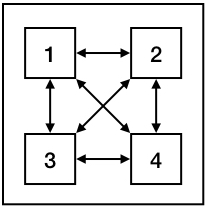
\includegraphics[width=0.75\textwidth]{local}
		\end{center}
	\end{column}
	\begin{column}{0.5\textwidth}  %%<--- here
		\vspace{-1.5em}
		\begin{center}
			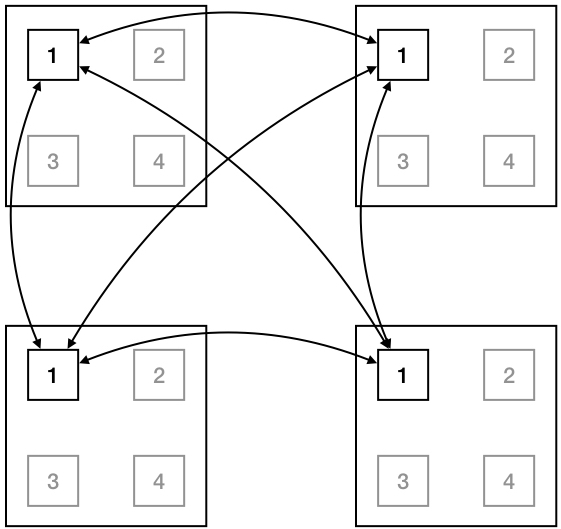
\includegraphics[width=0.9\textwidth]{remote}
		\end{center}
	\end{column}
\end{columns}

\end{frame}

%----------------------------------------------------------------------------------------

\begin{frame}
\frametitle{Node Local Node Remote}


\begin{columns}
	\begin{column}{0.5\textwidth}
		\textbf{Node Local Node Remote}
		\begin{itemize}
			\item Further partition $\mathcal{P}$ by \emph{layers}
			\begin{itemize}
				\item Set of (\# cores) nodes
			\end{itemize}
		\end{itemize}
	\end{column}
	\begin{column}{0.5\textwidth}  %%<--- here
		\begin{enumerate}
			\item Exchange locally	
			\item Forward remotely
			\item Forward locally
		\end{enumerate}
	\end{column}
\end{columns}

\begin{table}
\begin{tabular}{C|C}
	\hline
	\textbf{Intra-Layer Remote Route} & \textbf{Inter-Layer Remote Route} \\
	\hline
\end{tabular}
\end{table}
%
\vspace{-1.0em}
%
\begin{columns}
	\begin{column}{0.5\textwidth}
		\begin{center}
			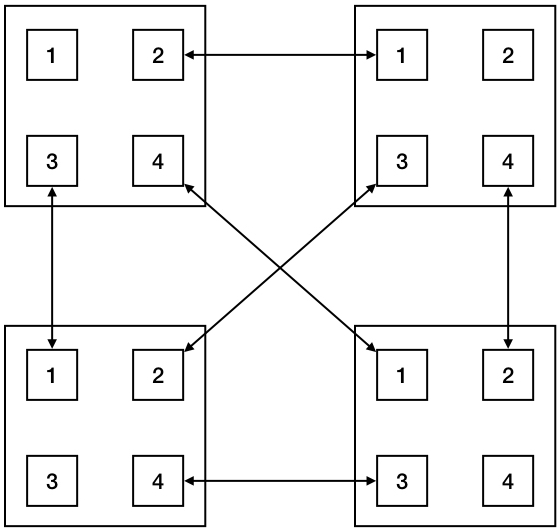
\includegraphics[width=0.9\textwidth]{intra_layer_nlnr}
		\end{center}
	\end{column}
	\begin{column}{0.5\textwidth}  %%<--- here
		\begin{center}
			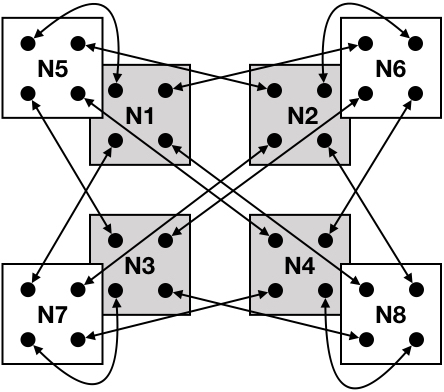
\includegraphics[width=0.9\textwidth]{inter_layer_nlnr}
		\end{center}
	\end{column}
\end{columns}

\end{frame}

%----------------------------------------------------------------------------------------

\begin{frame}
\frametitle{Validation of Claims}


\begin{figure}
	\begin{center}
		\begin{subfigure}{0.49\linewidth}
			\centerline{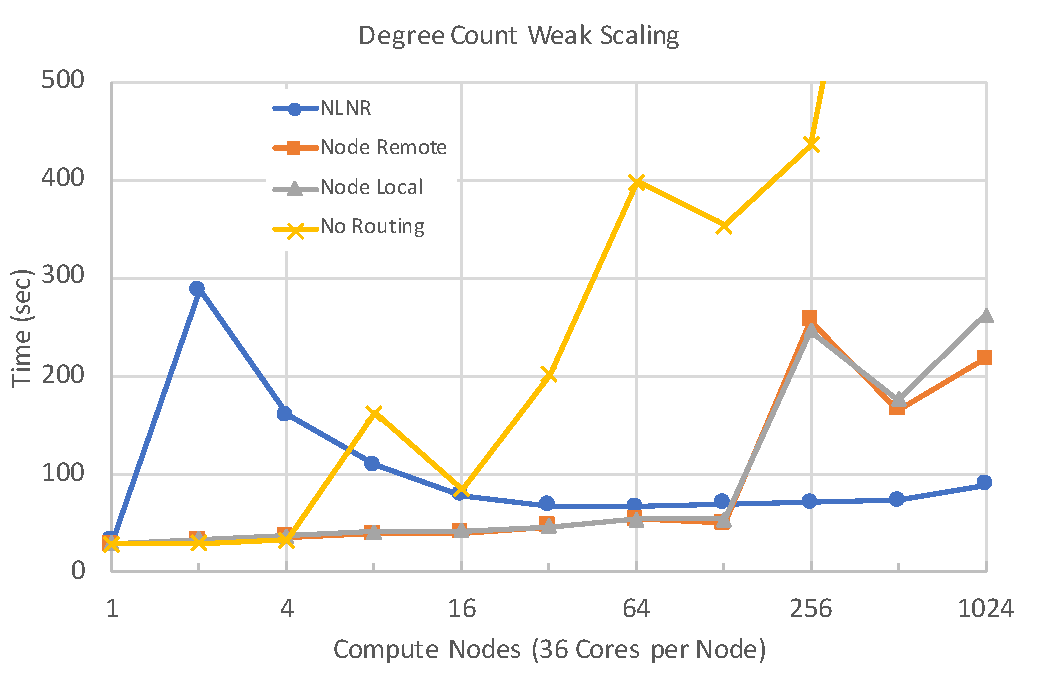
\includegraphics[width=1.0\columnwidth]{degree_weak_scaling}}
			\caption{Weak scaling. \label{fig:degree_weak_scaling}}
		\end{subfigure}
		\begin{subfigure}{0.49\linewidth}
			\centerline{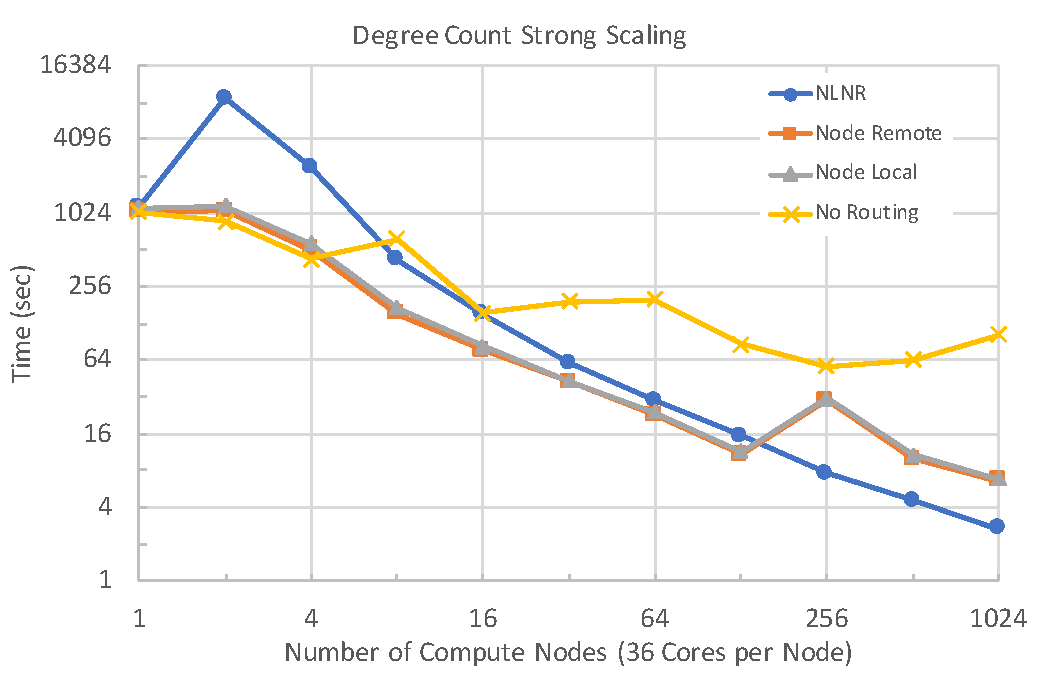
\includegraphics[width=1.0\columnwidth]{degree_strong_scaling}}
			\caption{Strong scaling \label{fig:degree_strong_scaling}}
		\end{subfigure}
		\caption{Weak and strong scaling wall time experiments for degree counting, as the number of nodes $N$ varies from 1 up to 1024.
			Weak scaling experiments (a) assumed a universe of $N2^{28}$ vertices and sampled a total of $N2^{32}$ edges.
			Strong scaling experiments (b) assumed a universe of $2^{32}$ vertices and sampled a total of $2^{37}$ edges. 
			Edge samplings uniformly sample two vertices without replacement from the universe of vertices.
			In all experiments mailbox sizes are fixed at $2^{18}$ messages.
			\label{fig:degree_scaling}}
	\end{center}
\end{figure}


%\begin{columns}
%\begin{column}{0.3\textwidth}
%	\textbf{Experiment}
%	\begin{itemize}
%		\item 20B message exchange
%		\begin{itemize}
%			\item Destination sampled from Pareto distribution
%			\item Batch size is maximum $|\mathcal{S}[P]|$
%		\end{itemize}
%		\item Run on quartz @ LLNL
%	\end{itemize}
%\end{column}
%\begin{column}{0.7\textwidth}  %%<--- here
%\begin{center}
%	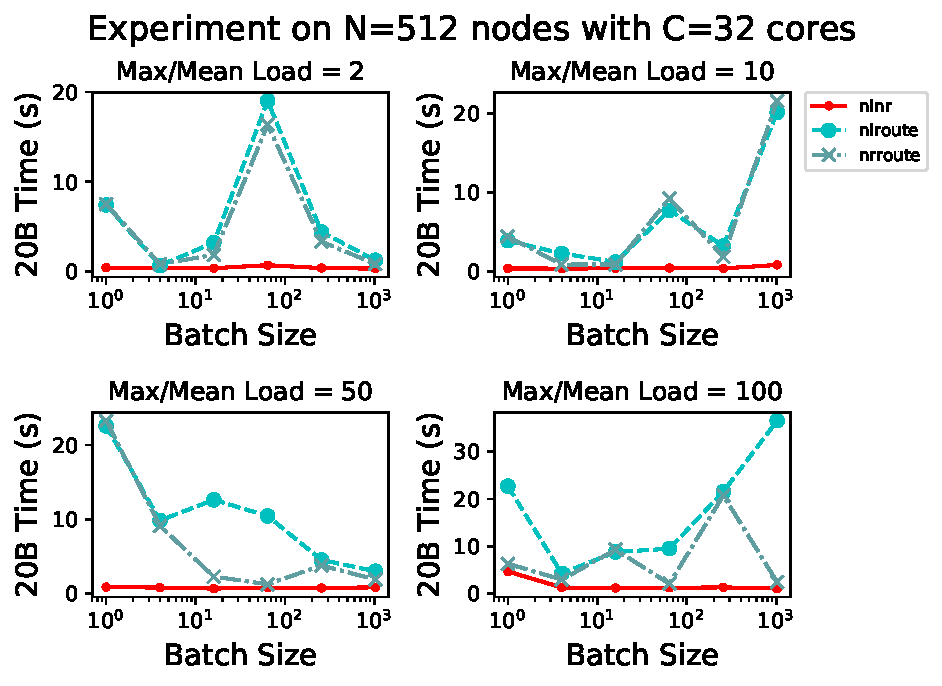
\includegraphics[width=1.0\textwidth]{512_32}
%\end{center}
%\end{column}
%
%\end{columns}
%
%\begin{block}{}
%	\begin{center}
%		NLNR exhibits best scaling, NR best with fewer nodes
%	\end{center}
%\end{block}

\end{frame}

%----------------------------------------------------------------------------------------

\begin{frame}
\frametitle{Implementation Details}


\textbf{\algoname{YGM} C++/MPI Library}
\begin{itemize}
	\item Authored by myself, Trevor Steil (UMN), and Roger Pearce (LLNL)
	\item Simple API for handling pseudo-asynchronous communication
	\begin{itemize}
		\item Clients need only specify receive behavior
	\end{itemize}
%	\item Supports message serialization for arbitrary, variable-length messages
	\item Supports LLNL Projects
	\begin{itemize}
		\item HavoqGT (graph challenge \& pattern matching)
		\item Sierra 42 - largest scale to date graph 500 ($\sim 70$T edges)
		\item Possibly more in the future
		\begin{itemize}
			\item e.g. Eccentricity
		\end{itemize}
	\end{itemize}
	\item Improvements over legacy HavoqGT routing
	\begin{itemize}
		\item Flow control via pseudo-asynchronicity 
		\item NLNR more scalable
		\item Variable length messages
	\end{itemize}
%	\item Useful for not just vertex-centric algorithms, but any algorithm with asymmetric computational and communication load
\end{itemize}

\begin{block}{}
	\begin{center}
		\algoname{YGM} to be open sourced, submitted to IPDPS 2019 workshop
	\end{center}
\end{block}

\end{frame}


%----------------------------------------------------------------------------------------
%----------------------------------------------------------------------------------------
\section{\algoname{DegreeSketch} and Local Triangle Count Heavy Hitters}
%----------------------------------------------------------------------------------------
%----------------------------------------------------------------------------------------

\againframe<6>{overview}

%----------------------------------------------------------------------------------------

\begin{frame}
\frametitle{Motivation: Local $t$th Neighborhood Size}

\textbf{The Problem}:
\begin{itemize}
	\item $t$th neighborhood important for applications, e.g. effective diameter, load balancing, edge prediction, and probabilistic distance estimation
	\begin{itemize}
		\item Exact computation expensive!
	\end{itemize}
	\item Neighborhood Functions:
\end{itemize}
%
\vspace{-0.5em}
\begin{align*}
	\mathcal{C}^{\algoname{Nbhd}}_t(x) 
	&= |\{y \in \mathcal{V} | d_\mathcal{G}(x, y) < t\}| 
	& \textnormal{local $t$th neighborhood} \\
	\mathcal{N}(t)  
	&=  |\{(x, y) \in \mathcal{V} \times \mathcal{V} | d_\mathcal{G}(x, y) < t\}|
	& \textnormal{(global) $t$th neighborhood}  \\
	&= \sum_{x \in \mathcal{V}} \mathcal{C}^{\algoname{Nbhd}}_t(x)  &
\end{align*}
%\vspace{-1.0em}
%
\textbf{Existing Approximate Solutions}:
\begin{itemize}
	\item ANF algorithm \cite{palmer2002anf}
	\item HyperANF algorithm \cite{boldi2011hyperanf}
\end{itemize}


\end{frame}

%----------------------------------------------------------------------------------------

\begin{frame}
\frametitle{Approach: \algoname{DegreeSketch} via Cardinality Sketches}


\begin{columns}
\begin{column}{0.65\textwidth}
	\textbf{Idea}: Sketch and iteratively merge adjacency sets
	\begin{itemize}
		\item Cardinality sketches summarize set size
		\item Supports approximate union operation $\widetilde{\cup}$
		\item Assume some partitioning $f : \mathcal{V} \rightarrow \mathcal{P}$
		\item Distributed data structure $\mathcal{D}$
		\begin{itemize}
			\item $\mathcal{D}[x]$ holds cardinality sketch for $x \in \mathcal{V}$
			\item $|\mathcal{D}[x]|$ estimates $\mathbf{d}_x$
		\end{itemize}
		\item Let $\mathcal{D}^1[x] = \mathcal{D}[x]$ 
		\item Set $\mathcal{D}^k[x] = \widetilde{\bigcup}_{y: xy \in \mathcal{E}} \mathcal{D}^{k-1}[y]$
		\item Then $\widetilde{\mathcal{C}}^{\algoname{Nbhd}}_t(x) = | \mathcal{D}^t[x]|$ and 
				$\widetilde{\mathcal{N}}(t) = \sum_{x \in \mathcal{V}} \widetilde{\mathcal{C}}^{\algoname{Nbhd}}_t(x)$
	\end{itemize}
\end{column}
\begin{column}{0.35\textwidth}  %%<--- here
	\begin{center}
		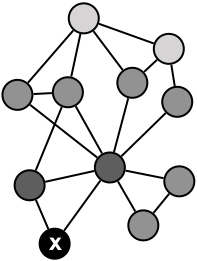
\includegraphics[width=1.0\textwidth]{nbhd_fig}
	\end{center}
\end{column}

\end{columns}


\end{frame}


%----------------------------------------------------------------------------------------

\begin{frame}
\frametitle{\algoname{HyperLogLog} Cardinality Sketches}

\begin{dynblock}
% l2 sampling
\opaqueblock<1>{
%
\textbf{\algoname{HLL} cardinality sketches} \\
Maintain $r = 2^p$ 6-bit registers $M$ and a 64-bit hash function $h$
\begin{itemize}
\item Insert $x$: let $i = \langle x_1, \dots, x_p \rangle$ and $w = \langle x_{p+1}, \dots, x_{64} \rangle$ 
\item $\rho(w) = $ initial zero bits of $w$ plus 1
\item $M_i = \max \{ M_i, \rho(w) \}$
\item Estimator derives from harmonic mean of $M$
\end{itemize}
%
}
\invblock<2->

% Second block
\opaqueblock<2->[0.6\textwidth]{
%
\vspace{-0.5cm}
%
\begin{center}
Outputs $\widetilde{C}$ such that for cardinality C, w.h.p. $| C - \widetilde{C} | \leq \frac{1.04}{\sqrt{r}} C$ \cite{flajolet2007hyperloglog}
\end{center}
}
\end{dynblock}



\begin{dynblock}
% rank-k approximation
\opaqueblock<3>{
%
\begin{tabular*}{\textwidth}{l @{\extracolsep{\fill}} r}
\textbf{Useful improvements}  & 
%[CW09]
\end{tabular*}
%
\vspace{-0.5cm}
%
\begin{itemize}
	\item Native union operator (elementwise maximum)
	\item Various improved harmonic \cite{heule2013hyperloglog, qin2016loglog} and maximum likelihood estimators \cite{xiao2017better, lang2017back, ertl2017new}
	\item Sparsification for low cardinality sets \cite{heule2013hyperloglog}
	\item Compression to 4 and 3 bit registers \cite{xiao2017better}
	\item Intersection estimators \cite{ting2016towards, cohen2017minimal, ertl2017new}
\end{itemize}
}

\end{dynblock}




\end{frame}


%----------------------------------------------------------------------------------------

\begin{frame}[label = accumulation]
\frametitle{\algoname{DegreeSketch} Accumulation} % Table of contents slide, comment this block out to remove it

\begin{center}
\only<1>{
		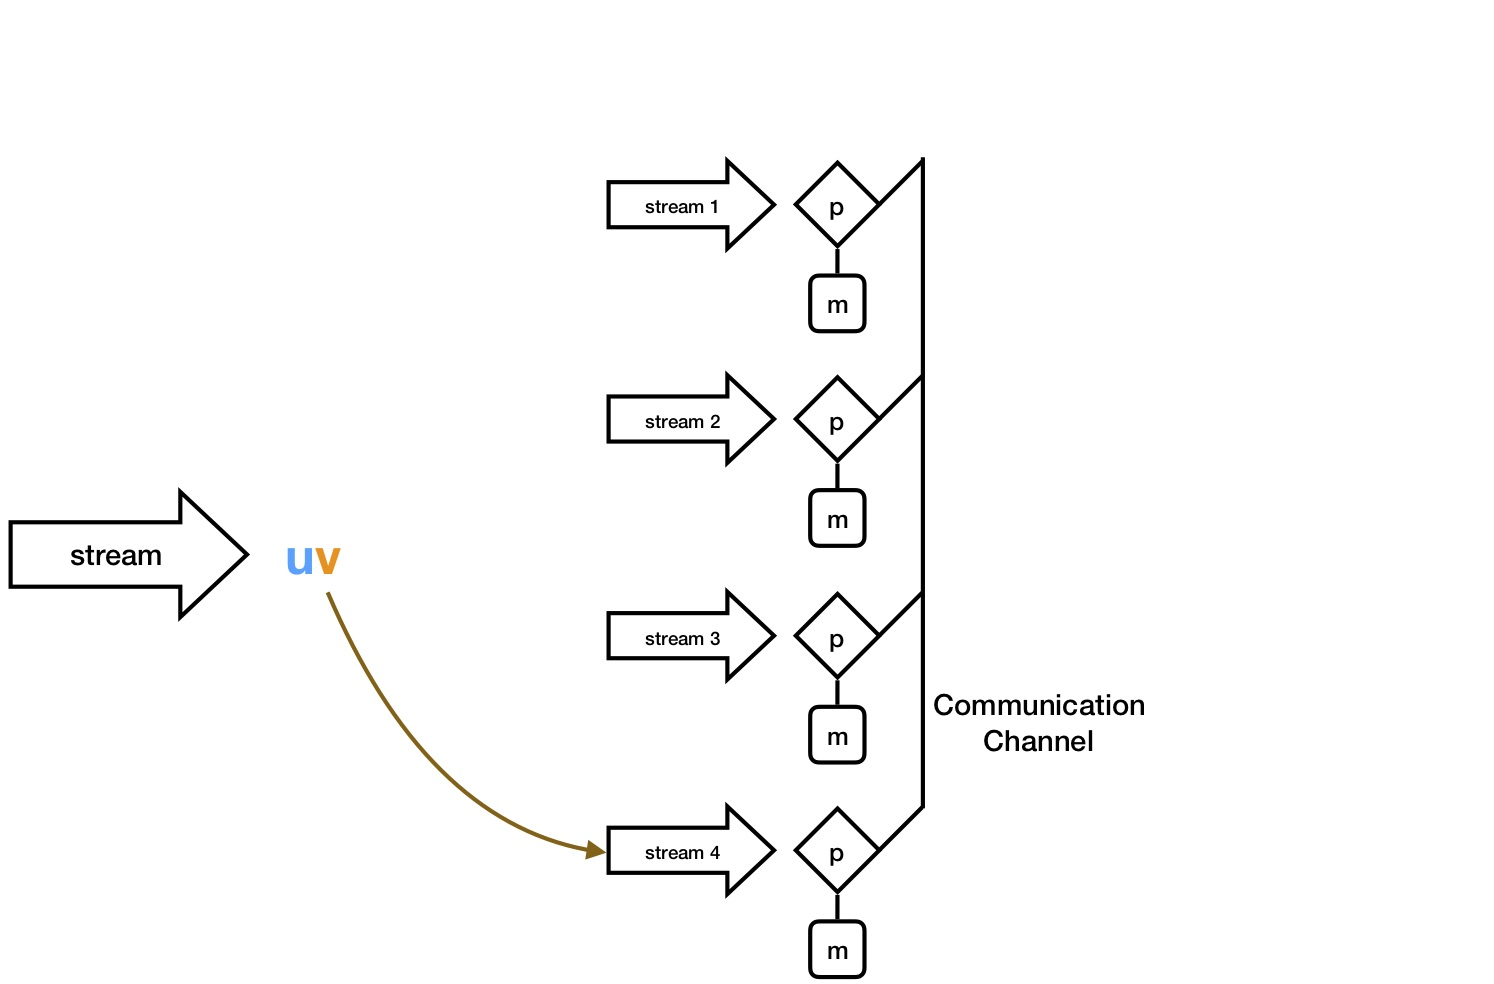
\includegraphics[width=0.85\textwidth]{ingest_1}
}
\only<2>{
		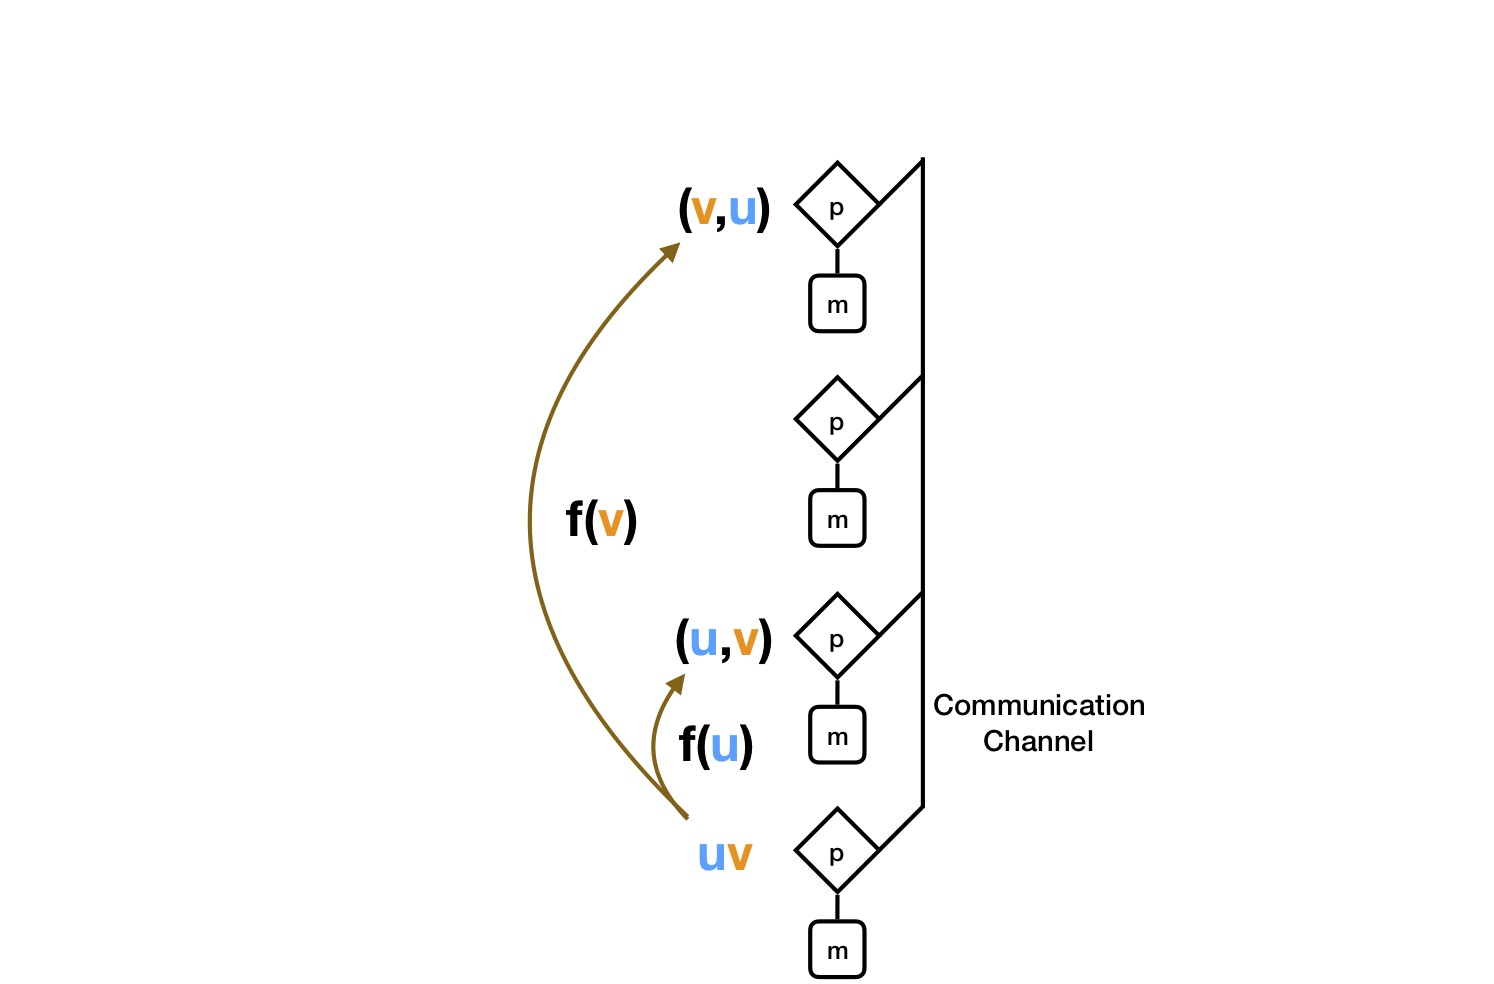
\includegraphics[width=0.85\textwidth]{ingest_2}
}
\only<3>{
		\includegraphics[width=0.85\textwidth]{ingest_3}
}
\end{center}

\begin{block}{}
\begin{center}
\only<1>{
	Partition stream across $\mathcal{P}$
}
\only<2>{
	Distribute edges to endpoint owners
}
\only<3>{
	Insert into $\mathcal{D}$ for each vertex
}
\end{center}
\end{block}

\end{frame}

%----------------------------------------------------------------------------------------

\begin{frame}[label = query]
\frametitle{\algoname{DegreeSketch} Neighborhood Update} % Table of contents slide, comment this block out to remove it

\begin{center}
\only<1>{
		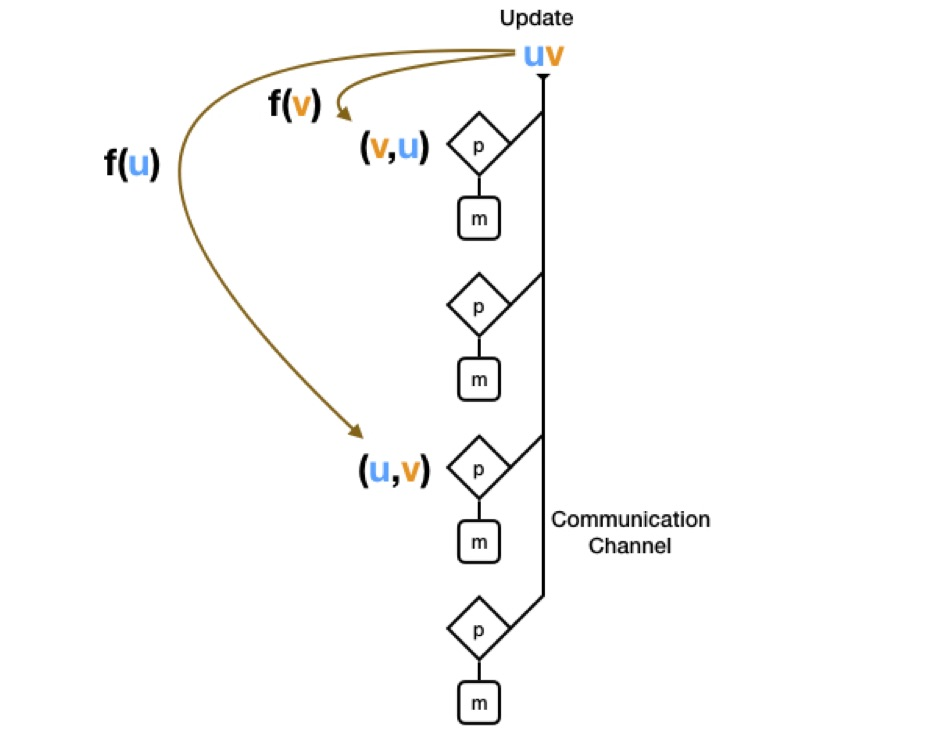
\includegraphics[width=0.7\textwidth]{nbhd_update_1}
}
\only<2>{
		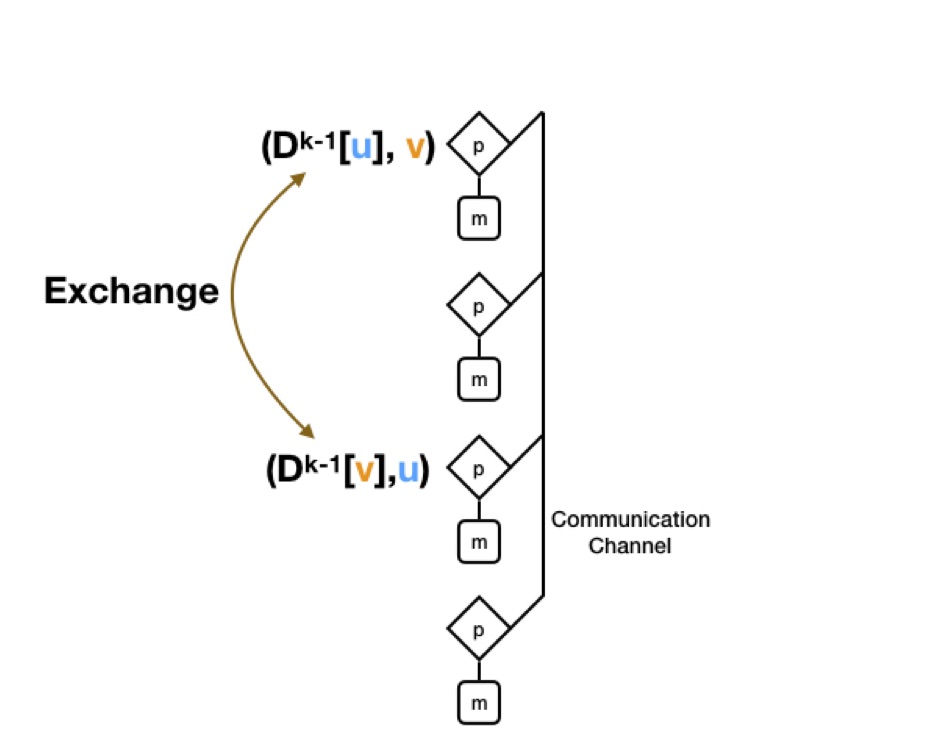
\includegraphics[width=0.7\textwidth]{nbhd_update_2}
}
\only<3>{
		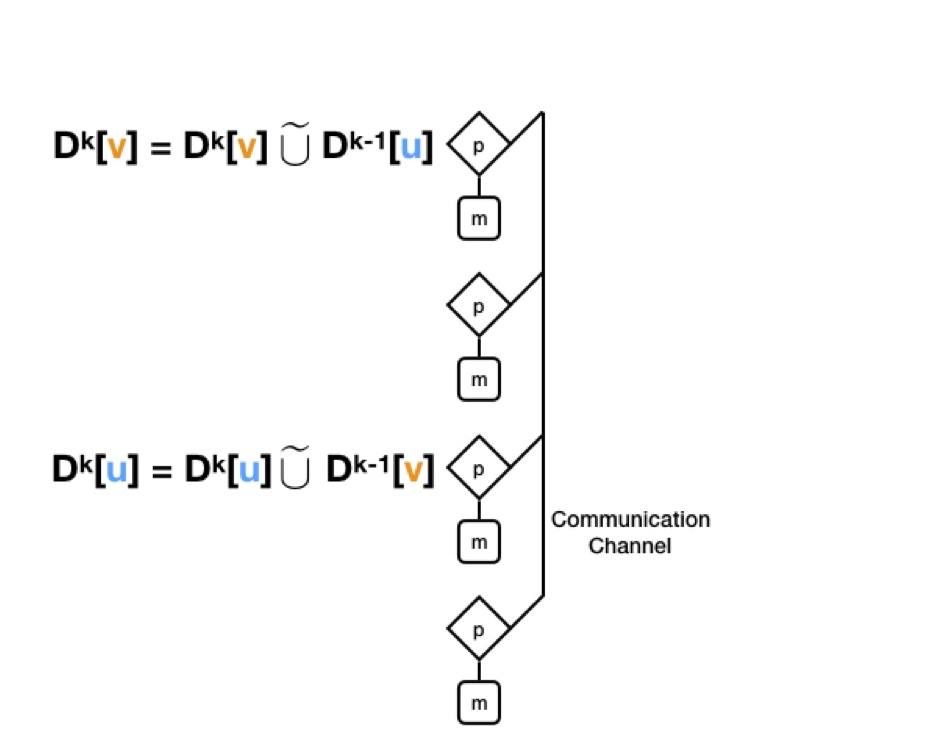
\includegraphics[width=0.7\textwidth]{nbhd_update_3}
}
\only<4>{
		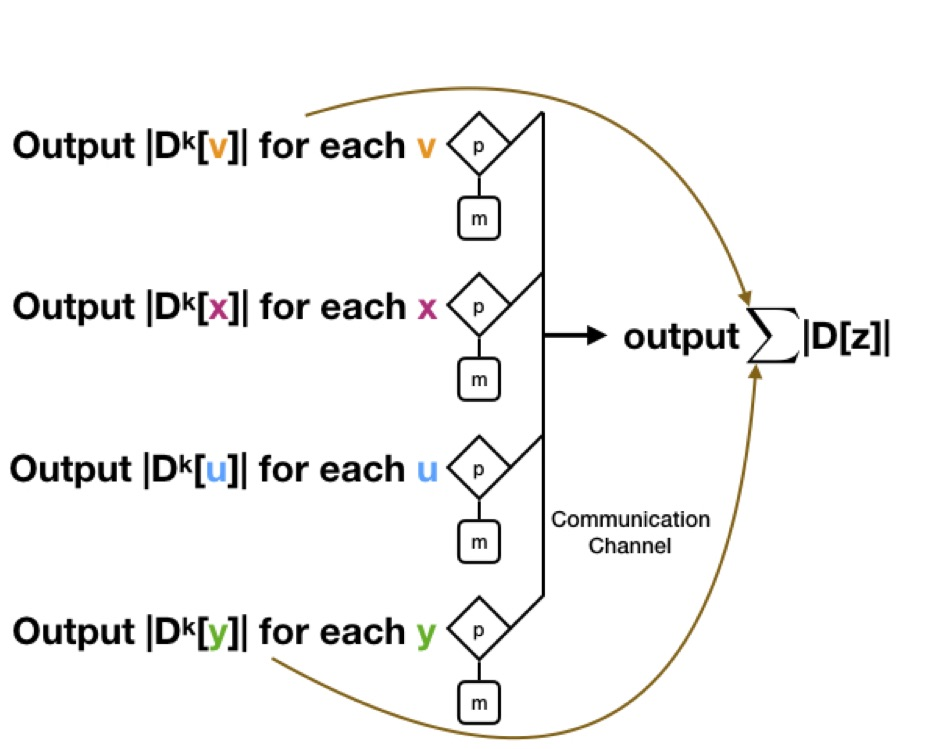
\includegraphics[width=0.7\textwidth]{nbhd_update_4}
}
\end{center}

\begin{block}{}
\begin{center}
\only<1>{
	Updates route to each endpoint owner
}
\only<2>{
	Owners exchange ($k-1$)th skeches
}
\only<3>{
	$(k-1)$th sketches are merged into $k$th sketches
}
\only<4>{
	After $k$th pass, output all $k$th local and global estimates
}
\end{center}
\end{block}

\end{frame}

%----------------------------------------------------------------------------------------

\begin{frame}
\frametitle{Neighborhood Estimation: Correctness}

\begin{block}{Theorem 6.3.1}
Let $\mu_{r, n}$ and $\eta_{r, n}$ be the multiplicative bias and standard deviation for \algoname{HLL}s given in Theorem 1 of \cite{flajolet2007hyperloglog}.
%, where $\mu_{r, n}$ is the sum of a small constant and an oscillating function of small amplitude. 
The output $\widetilde{\mathcal{N}}(t)$ and $\widetilde{\mathcal{C}}^{\algoname{Nbhd}}_t(x)$ for $x \in \mathcal{V}$ at the $t$-th iteration satisfies 
%
\begin{equation*}
	\frac{\E \left [ \widetilde{\mathcal{N}}(t) \right ]}{\mathcal{N}(t)} 
	= \frac{\E \left [ \widetilde{\mathcal{C}}^{\algoname{Nbhd}}_t(x) \right ]}{\mathcal{C}^{\algoname{Nbhd}}_t(x)} 
	= \mu_{r, n} 
	\textnormal{ for $n \rightarrow \infty$,}
\end{equation*}
%
i.e. they are nearly unbiased.
%where $\delta_1(n)$ is the same as in \cite{flajolet2007hyperloglog} Theorem 1, and $|\delta_1(x)| < 5 \cdot 10^{-5}$ when $r \geq 16$.

Furthermore, both also have standard deviation bounded by $\eta_{r,n}$.
%the output $\widetilde{\mathcal{C}}^{\algoname{Nbhd}}_t(x)$ for $x \in \mathcal{V}$ has the standard deviation $\eta_r$ given by \cite{flajolet2007hyperloglog}, which is also shared by $\widetilde{N}(t)$. 
That is, 
%
\begin{equation*}
	\frac{\sqrt{\Var \left [ \widetilde{\mathcal{N}}(t)\right ]}}{\mathcal{N}(t)} \leq \eta_{r, n}
	\textnormal{ and }
	\frac{\sqrt{\Var \left [ \widetilde{\mathcal{C}}^{\algoname{Nbhd}}_t(x) \right ]}}{\mathcal{C}^{\algoname{Nbhd}}_t(x)} \leq \eta_{r, n}
\end{equation*}
%
%Implementing Algorithm~\ref{alg:ds:anf} with \algoname{HyperLogLog} sketches requires $\widetilde{O}(m)$ time and bits of communication, and only $O(n ( \varepsilon^{-1}\log\log n + \log n))$ space.
\end{block}

\end{frame}


%----------------------------------------------------------------------------------------

\begin{frame}
\frametitle{Neighborhood Estimation: Correctness}

\begin{block}{Proof of Theorem 6.3.1}
For each $x$, $\widetilde{\mathcal{C}}^{\algoname{Nbhd}}_t(x) = |\mathcal{D}^k[x]|$, where $\mathcal{D}^k[x]$ is a union of \algoname{HLL}s, into which every $y$ such that $d(x,y) < t$ is inserted. 
Thus by Theorem 1 of \cite{flajolet2007hyperloglog}, 
%
\begin{align*}
%\E \left [ \left | \mathcal{D}^k[x] \right | \right ] 
\E \left [ \widetilde{\mathcal{C}}^{\algoname{Nbhd}}_t(x) \right ] 
&= \mu_{r,n} \mathcal{C}^{\algoname{Nbhd}}_t(x) \\
%\sqrt{\Var \left [ \left | \mathcal{D}^k[x] \right | \right ]} 
\sqrt{\Var \left [ \widetilde{\mathcal{C}}^{\algoname{Nbhd}}_t(x) \right ]} 
&= \eta_{r,n} \mathcal{C}^{\algoname{Nbhd}}_t(x).
\end{align*}
%
Thus, 
\begin{align*}
\E \left [ \widetilde{N}(t) \right ] 
%= \sum_{x \in \mathcal{V}} \E \left [ \left | \mathcal{D}^k[x] \right | \right ]  
= \sum_{x \in \mathcal{V}} \E \left [ \widetilde{\mathcal{C}}^{\algoname{Nbhd}}_t(x) \right ]  
= \mu_{r, n} \sum_{x \in \mathcal{V}} \mathcal{C}^{\algoname{Nbhd}}_t(x)  
= \mu_{r,n} \mathcal{N}(t),
\textnormal{ and} \\
%\end{equation*}
%
%and
%
%\begin{equation*}
\sqrt{\Var \left [ \widetilde{N}(t) \right ]} 
%\leq \sum_{x \in \mathcal{V}} \sqrt{\Var \left [ \left | \mathcal{D}^k[x] \right | \right ]}  
\leq \sum_{x \in \mathcal{V}} \sqrt{\Var \left [ \widetilde{\mathcal{C}}^{\algoname{Nbhd}}_t(x) \right ]}  
\leq \eta_{r, n} \sum_{x \in \mathcal{V}} \mathcal{C}^{\algoname{Nbhd}}_t(x)  
= \eta_{r, n} \mathcal{N}(t).
\end{align*}

\end{block}

\end{frame}


%----------------------------------------------------------------------------------------

\begin{frame}
\frametitle{Another Application: Local Triangle Counting}

\textbf{The Problem}:
\begin{itemize}
	\item Local triangle counting a common big data analytic
	\begin{itemize}
		\item Exact computation expensive $O \left ( m^{\frac{3}{2}} \right )$!
	\end{itemize}
	\item Recall
\end{itemize}
%
\vspace{-0.5em}
\begin{align*}
	\mathcal{C}^{\algoname{Tri}}(x) 
	&= |\{yz \in \mathcal{E} \mid xy, yz, xz \in \mathcal{E} \}| 
	& \textnormal{(vertex-local)} \\
	\mathcal{C}^{\algoname{Tri}}(xy) 
	&= |\{z \in \mathcal{E} \mid xy, yz, xz \in \mathcal{E} \}|
	& \textnormal{(edge-local)} 
\end{align*}
%\vspace{-1.0em}
%
\textbf{Existing Solutions}:
\begin{itemize}
	\item Many exact distributed algorithms \cite{arifuzzaman2013patric, pearce2017triangle}
	\item Many approximate streaming algorithms via sampling \cite{lim2015mascot, stefani2017triest}
	\item ... and some utilizing both models \cite{shin2018tri, shin2018dislr}
\end{itemize}


\end{frame}


%----------------------------------------------------------------------------------------

\begin{frame}
\frametitle{Approach: Semi-Streaming Intersection Method}


\begin{columns}
\begin{column}{0.65\textwidth}
	\textbf{Idea}: Intersection method, but using \algoname{DegreeSketch}
	\begin{itemize}
		\item Some cardinality sketches support a limited intersection operation $\widetilde{\cap}$
%		\begin{itemize}
%			\item High variance if intersection is small
%			\item Likely best performance on heavy hitters
%		\end{itemize}
		\item Affords edge- and vertex-local triangle count estimation
		\item Approximate intersection implementation rules out analytic verification \`a la neighborhood estimation
		\begin{itemize}
			\item Requires empirical evaluation		
		\end{itemize}
%		\item Large variance induced by low \emph{triangle density} and \emph{dominations}
%		\begin{itemize}
%			\item Triangle density = $\frac{\textnormal{\# triangles}}{\textnormal{\# possible triangles}}$
%			\item Domination = one sketch element-wise greater than the other
%		\end{itemize}
	\end{itemize}
\end{column}
\begin{column}{0.35\textwidth}  %%<--- here
	\begin{center}
		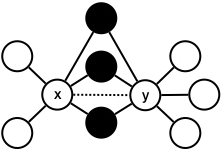
\includegraphics[width=1.0\textwidth]{edge_local}
	\end{center}
	\begin{center}
		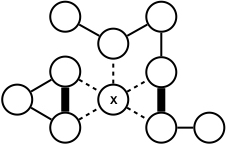
\includegraphics[width=1.0\textwidth]{vertex_local}
	\end{center}
\end{column}

\end{columns}


\end{frame}


%----------------------------------------------------------------------------------------

\begin{frame}
\frametitle{Set operation estimation with \algoname{HLL}s}

Streaming sets $X$ and $Y$ with \algoname{HLL}s $S_X$ and $S_Y$
\begin{columns}
\begin{column}{0.5\textwidth}
	\begin{itemize}
		\item $S_X \approx |X|$
		\item $S_Y \approx |Y|$
		\item $S_X \widetilde{\cup} S_Y \approx |X \cup Y|$
		\begin{itemize}
			\item Same error guarantees
		\end{itemize}
		\item $S_X \widetilde{\cap} S_Y \approx |X \cap Y|$
		\begin{itemize}
			\item High variance if $|X \cap Y|$ small
			\item Optimization arbitrary if $S_X \leq S_Y$ element-wise
		\end{itemize}
	\end{itemize}
\end{column}
\begin{column}{0.5\textwidth}  %%<--- here
	\begin{center}
		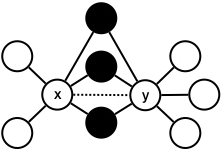
\includegraphics[width=1.0\textwidth]{edge_local}
	\end{center}
\end{column}

\end{columns}


\end{frame}

%----------------------------------------------------------------------------------------

\begin{frame}[label = query]
\frametitle{\algoname{DegreeSketch} Query} % Table of contents slide, comment this block out to remove it

\begin{center}
\only<1>{
		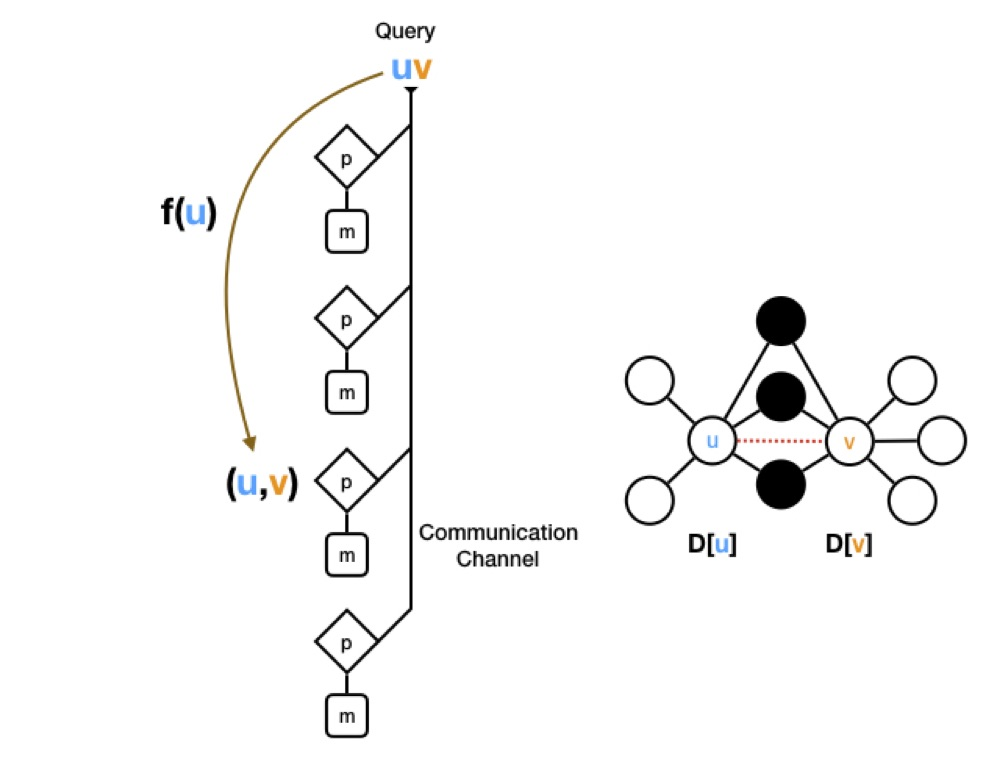
\includegraphics[width=0.72\textwidth]{query_1}
}
\only<2>{
		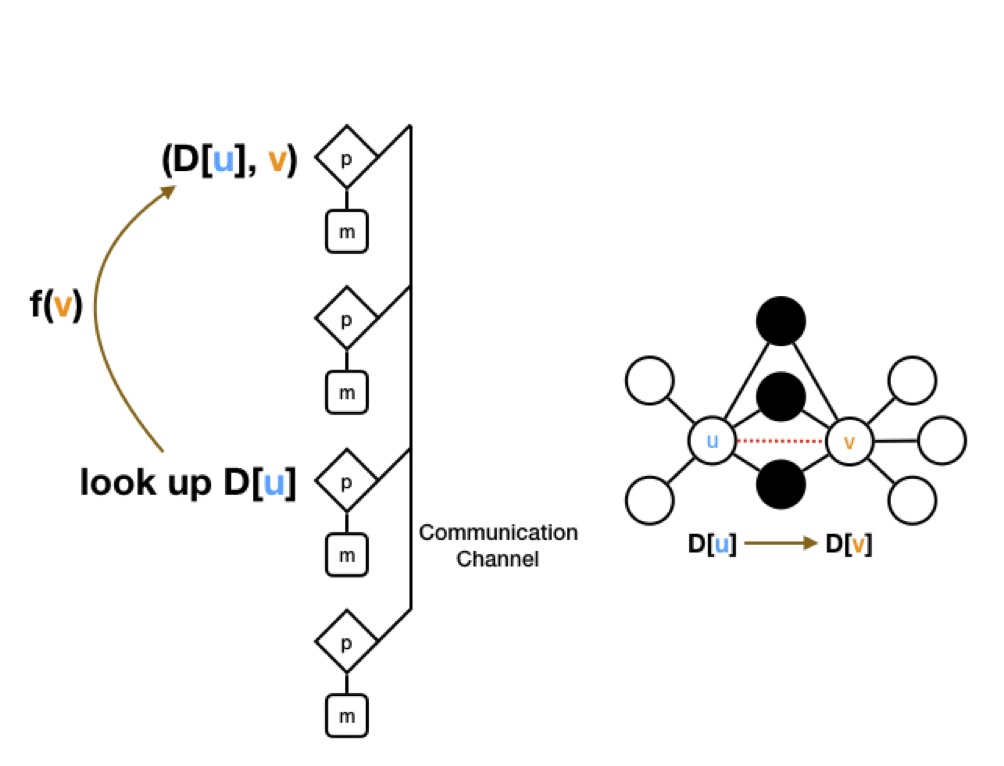
\includegraphics[width=0.72\textwidth]{query_2}
}
\only<3>{
		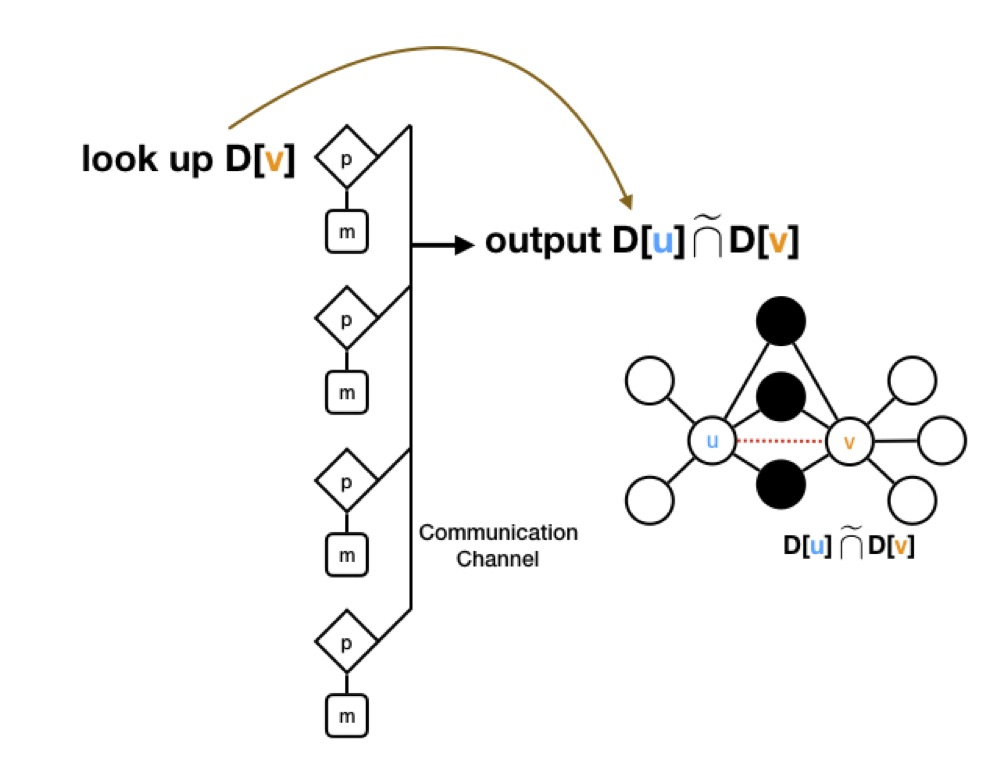
\includegraphics[width=0.72\textwidth]{query_3}
}
\end{center}

\begin{block}{}
\begin{center}
\only<1>{
	Query routes to one endpoint owner
}
\only<2>{
	Owner sends cardinality sketch to other endpoint owner
}
\only<3>{
	Final owner outputs intersection estimation
}
\end{center}
\end{block}

\end{frame}

%----------------------------------------------------------------------------------------



\begin{frame}
\frametitle{\algoname{DegreeSketch} and Triangle Counting}


%\begin{definition}[$\ell_p$-Sampling Sketch]
%A distribution $\Pi$  on $k \times n$ matrices so that if for any $v \in \mathbb{R}^n$, $S$ drawn from $\Pi$ is such that, given $Sv$, one can produce $i \in [n]$ sampled with probability $(1 \pm \varepsilon)\frac{|v_i|^p}{\|v\|_p}$
%\end{definition}

Assume a partition $f : \mathcal{V} \rightarrow \mathcal{P}$, and let $\mathcal{V}_P = \{v \in \mathcal{V} \mid f(v) = P\}$
\begin{itemize}
	\item Distribute $\algoname{DegreeSketch}$ $\mathcal{D}$ across $\mathcal{P}$
	\begin{itemize}
		\item $\mathcal{D}[v]$ holds a \algoname{HLL} for adjacency set of $v \in \mathcal{V}$
		\item $P$ holds $\mathcal{D}[v]$ for $v \in \mathcal{V}_P$
	\end{itemize}
	\item Accumulate $\mathcal{D}$ in one pass over $\sigma$
	\begin{itemize}
		\item Assume $P \in \mathcal{P}$	gets substream $\sigma_P$
		\item $P$ sends $xy \in \sigma_P$ to $f(x)$ and $f(y)$
		\item When $P$ gets $xy : x \in \mathcal{V}_P$, insert $y$ into $\mathcal{D}[x]$
		\begin{itemize}
			\item $\mathcal{D}[x]$ starts sparse and eventually saturates
		\end{itemize}
	\end{itemize}
	\item $\mathcal{D}$ can be queried after estimation, e.g.
	\begin{itemize}
		\item Estimate $\widetilde{\mathcal{C}}^{\algoname{Deg}}(v)  = \algoname{Estimate}(\mathcal{D}[v])$
		\item Estimate $\widetilde{\mathcal{C}}^{\algoname{Tri}}(uv) = \mathcal{D}[u] \widetilde{\cap} \mathcal{D}[v]$
		\begin{itemize}
			\item Involves communication if $f(u) \neq f(v)$
		\end{itemize}
		\item Estimate $\widetilde{\mathcal{C}}^{\algoname{Tri}}(v) = \frac{\sum_{uv \in \mathcal{E}} \widetilde{\mathcal{C}}^{\algoname{Tri}}(uv)}{2}$
		\begin{itemize}
			\item Requires second pass in general
		\end{itemize}
	\end{itemize}
\end{itemize}

\begin{block}{}
\begin{center}
$\widetilde{O}(m)$ time and communication and $\widetilde{O}(\varepsilon^{-2}n)$ space!
\end{center}
\end{block}

\end{frame}

%----------------------------------------------------------------------------------------

%\begin{frame}
%\frametitle{Edge-Local Triangle Count Heavy Hitters}
%
%\begin{algorithm}[H]
%\caption{Edge-Local Triangle Count Heavy Hitters}\label{alg:sublinear_kpath}
%\begin{algorithmic}[1]
%%\State $T \gets 2 \kappa^2 n^{1-2\alpha} \ln n$
%\State Accumulate $\mathcal{D}$ in distributed pass over $\sigma$
%\State $H_k \gets \textnormal{empty $k$-heap}$
%\State $T \gets 0$
%\ParFor{$xy \in \sigma_P$}  \qquad // second pass
%	\State Send $(\textnormal{E}, xy)$ to $f(x)$
%	\For {$(\textnormal{E}, xy) \in \mathcal{R}[P]$}
%		\State Send $(\textnormal{S}, xy, \mathcal{D}[x])$ to $f(y)$
%	\EndFor
%	\For {$(\textnormal{S}, xy, \mathcal{D}[x]) \in \mathcal{R}[P]$}
%		\State Insert $(xy, \mathcal{D}[x] \widetilde{\cap} \mathcal{D}[y])$ into $H_k$
%		\State $T \gets T + \mathcal{D}[x] \widetilde{\cap} \mathcal{D}[y]$
%	\EndFor
%\EndParFor
%\State $T \gets T / 2$
%\State Global accounting of $T$, $H_k$
%\State \Return $H_k$
%\end{algorithmic}
%\end{algorithm}
%
%
%
%\end{frame}


%----------------------------------------------------------------------------------------

\begin{frame}
\frametitle{Validation of Claims}

\begin{columns}
	\begin{column}{0.2\textwidth}
		\begin{block}{}
			HPEC graph challenge results
		\end{block}
		\begin{block}{}
			Good performance  on heavy hitters of \emph{most} graphs
		\end{block}
		\begin{block}{}
			Why do some graphs perform worse?
		\end{block}
	\end{column}
	\begin{column}{0.4\textwidth}
		\centerline{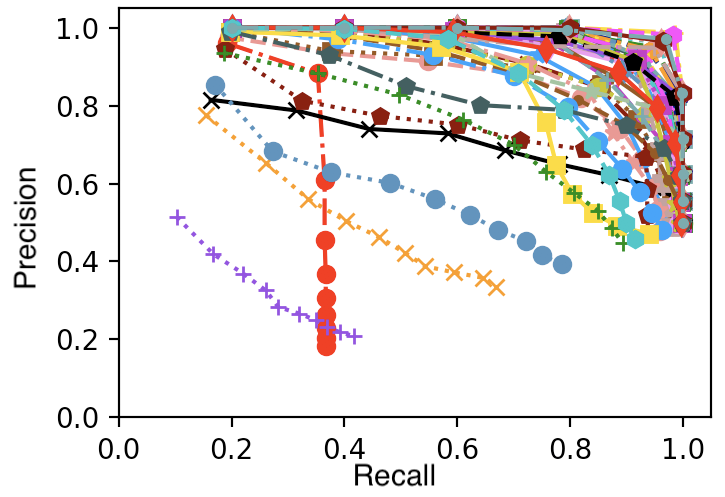
\includegraphics[width=1.0\columnwidth]{precision_vs_recall_top_10}}
		\centerline{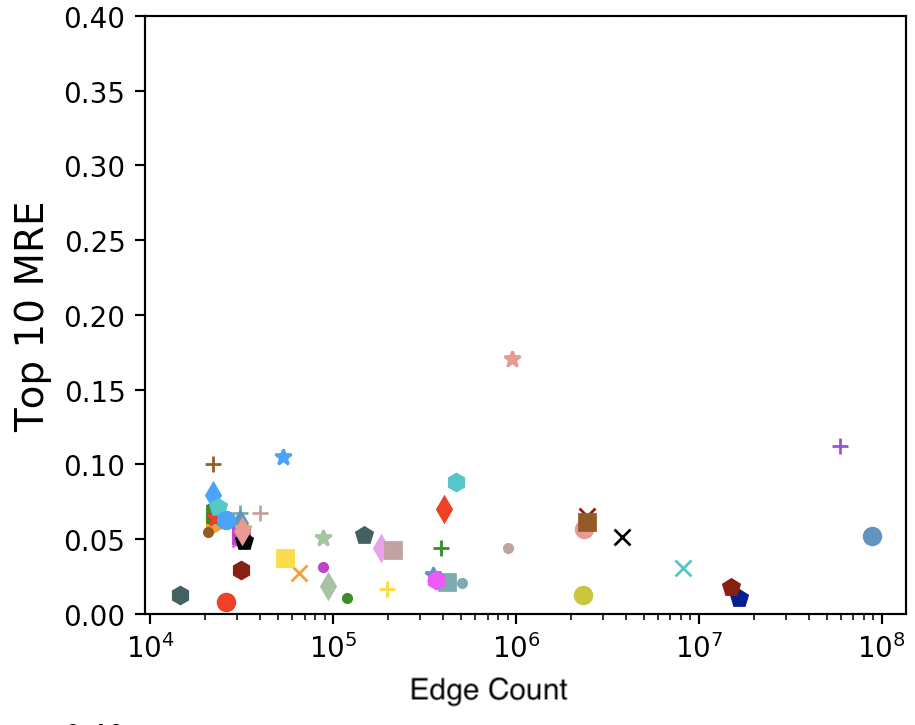
\includegraphics[width=1.0\columnwidth]{errs_vs_E_top_10}}
	\end{column}
	\begin{column}{0.4\textwidth}
		\centerline{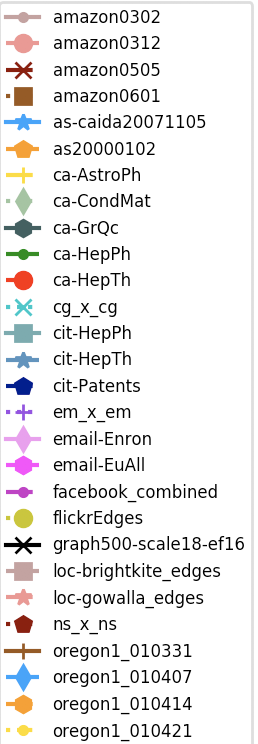
\includegraphics[width=0.5\columnwidth]{gc_legend_1}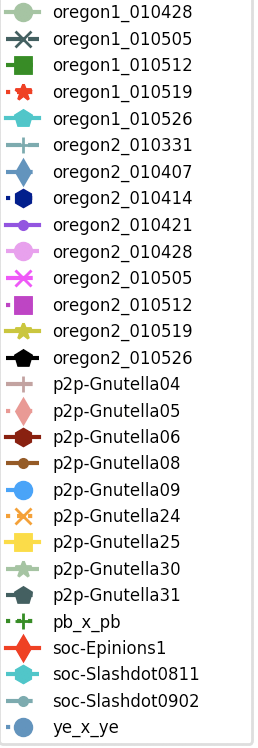
\includegraphics[width=0.5\columnwidth]{gc_legend_2}}
	\end{column}
\end{columns}

\end{frame}


%----------------------------------------------------------------------------------------

%\begin{frame}
%\frametitle{Validation of Claims: Relative Error}
%
%\centerline{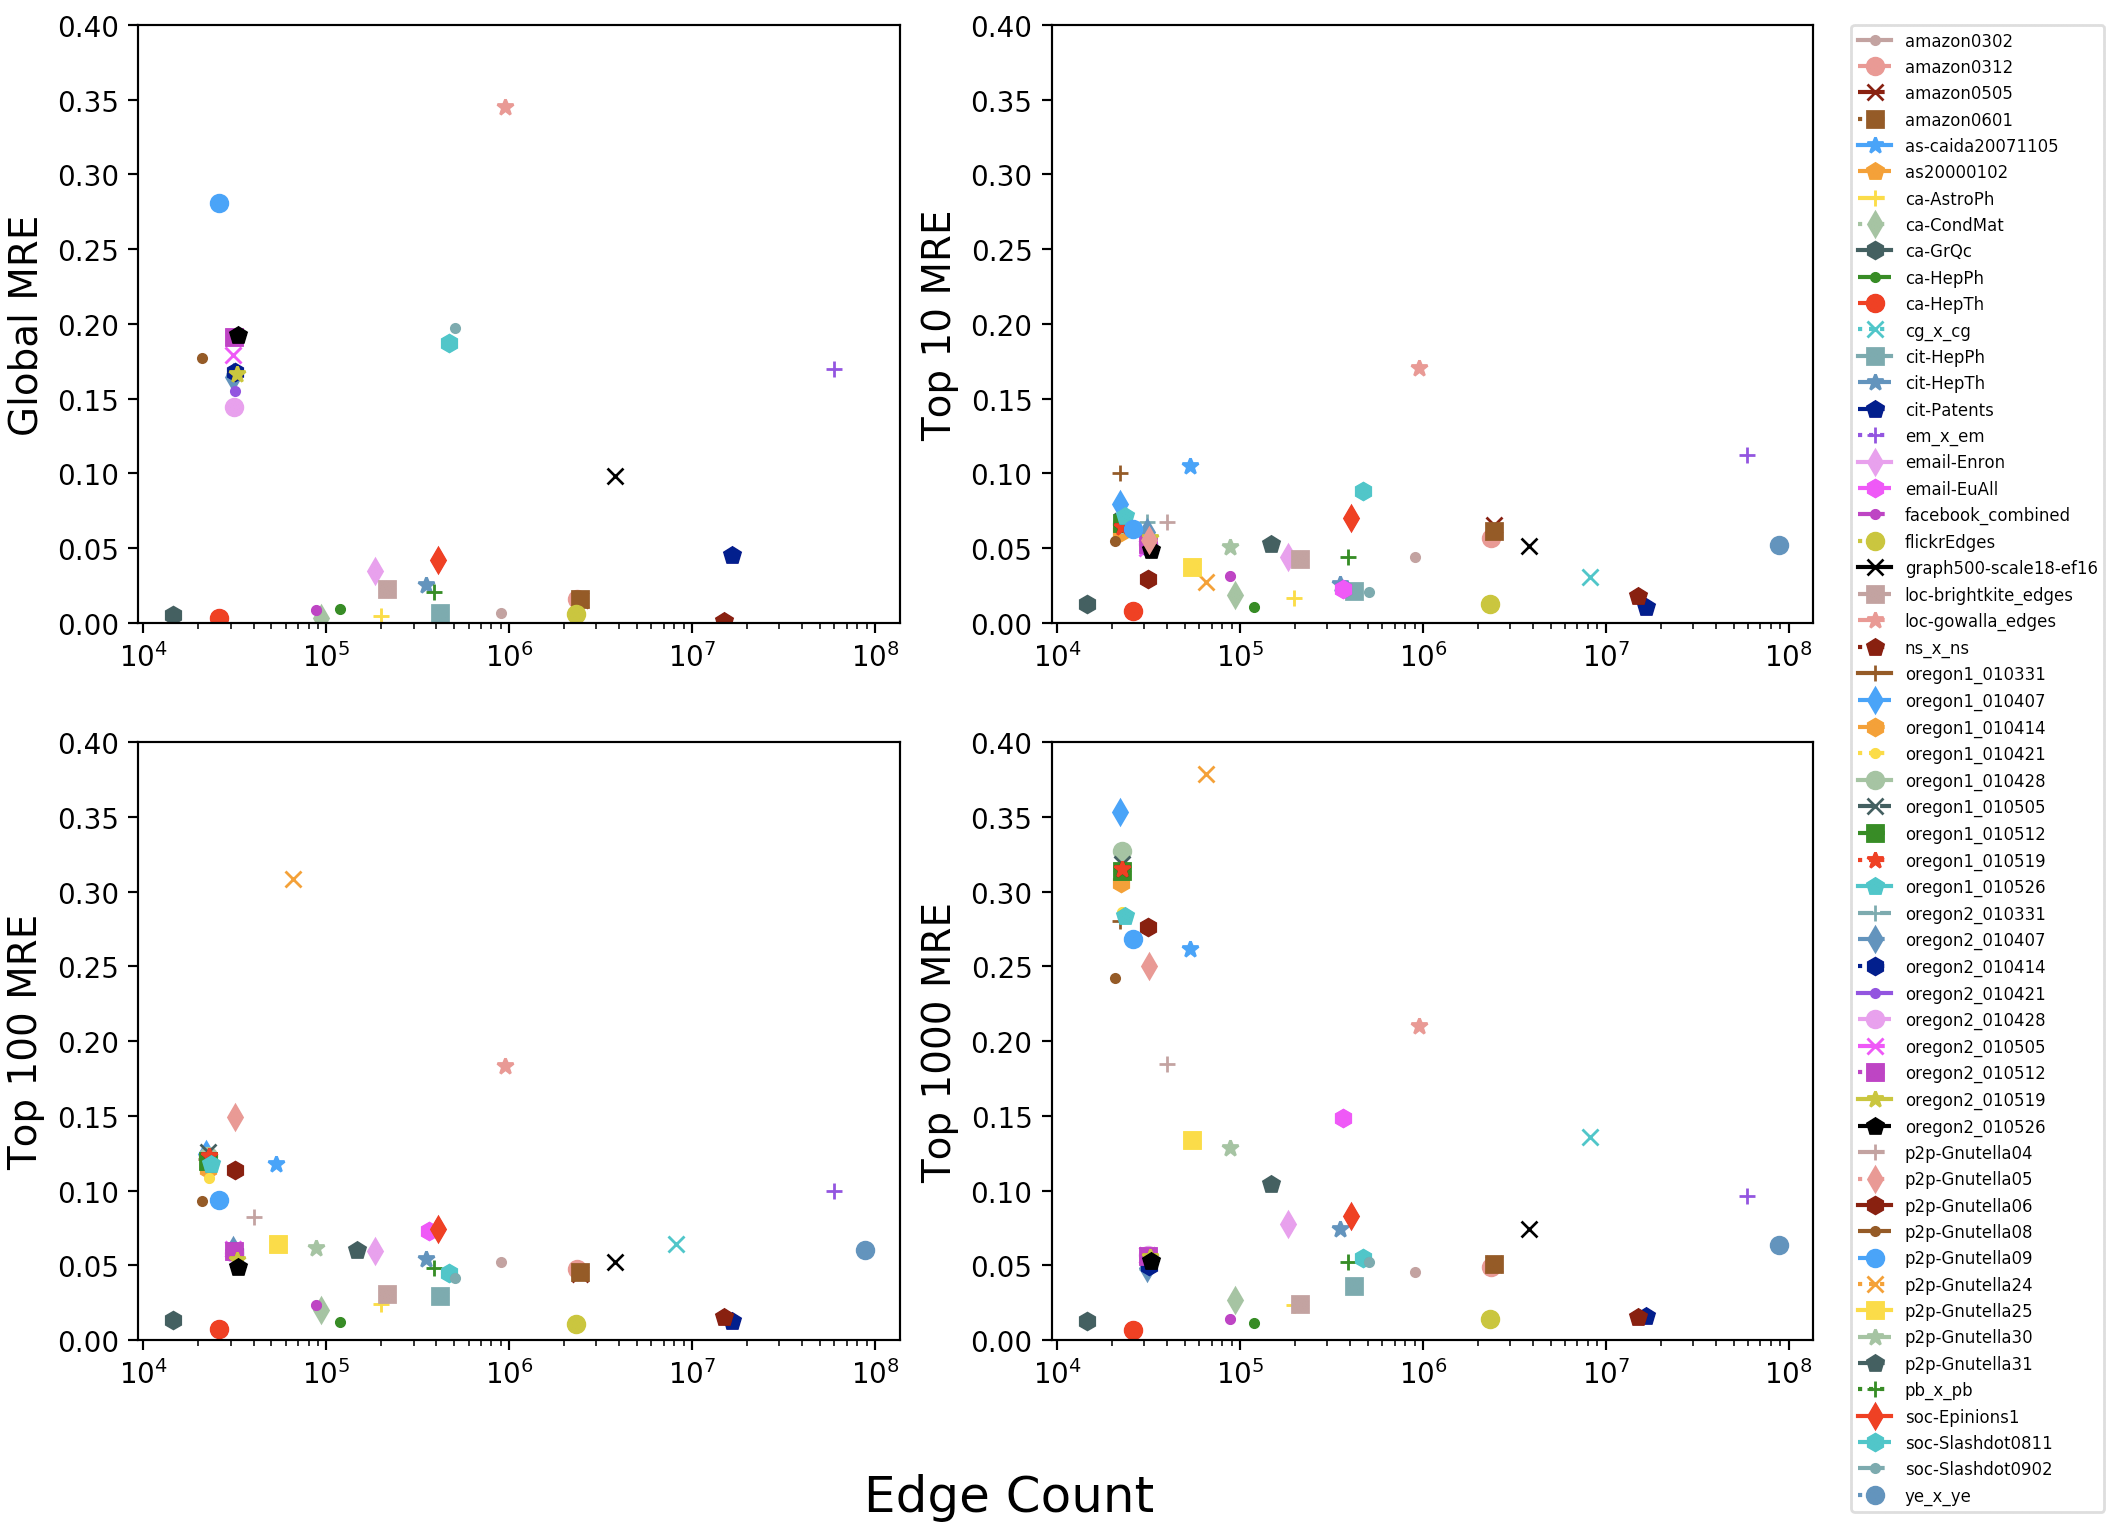
\includegraphics[width=0.9\columnwidth]{errs_vs_E}}
%
%\end{frame}

%----------------------------------------------------------------------------------------

\begin{frame}
\frametitle{Heavy Hitter Distributions}

\centerline{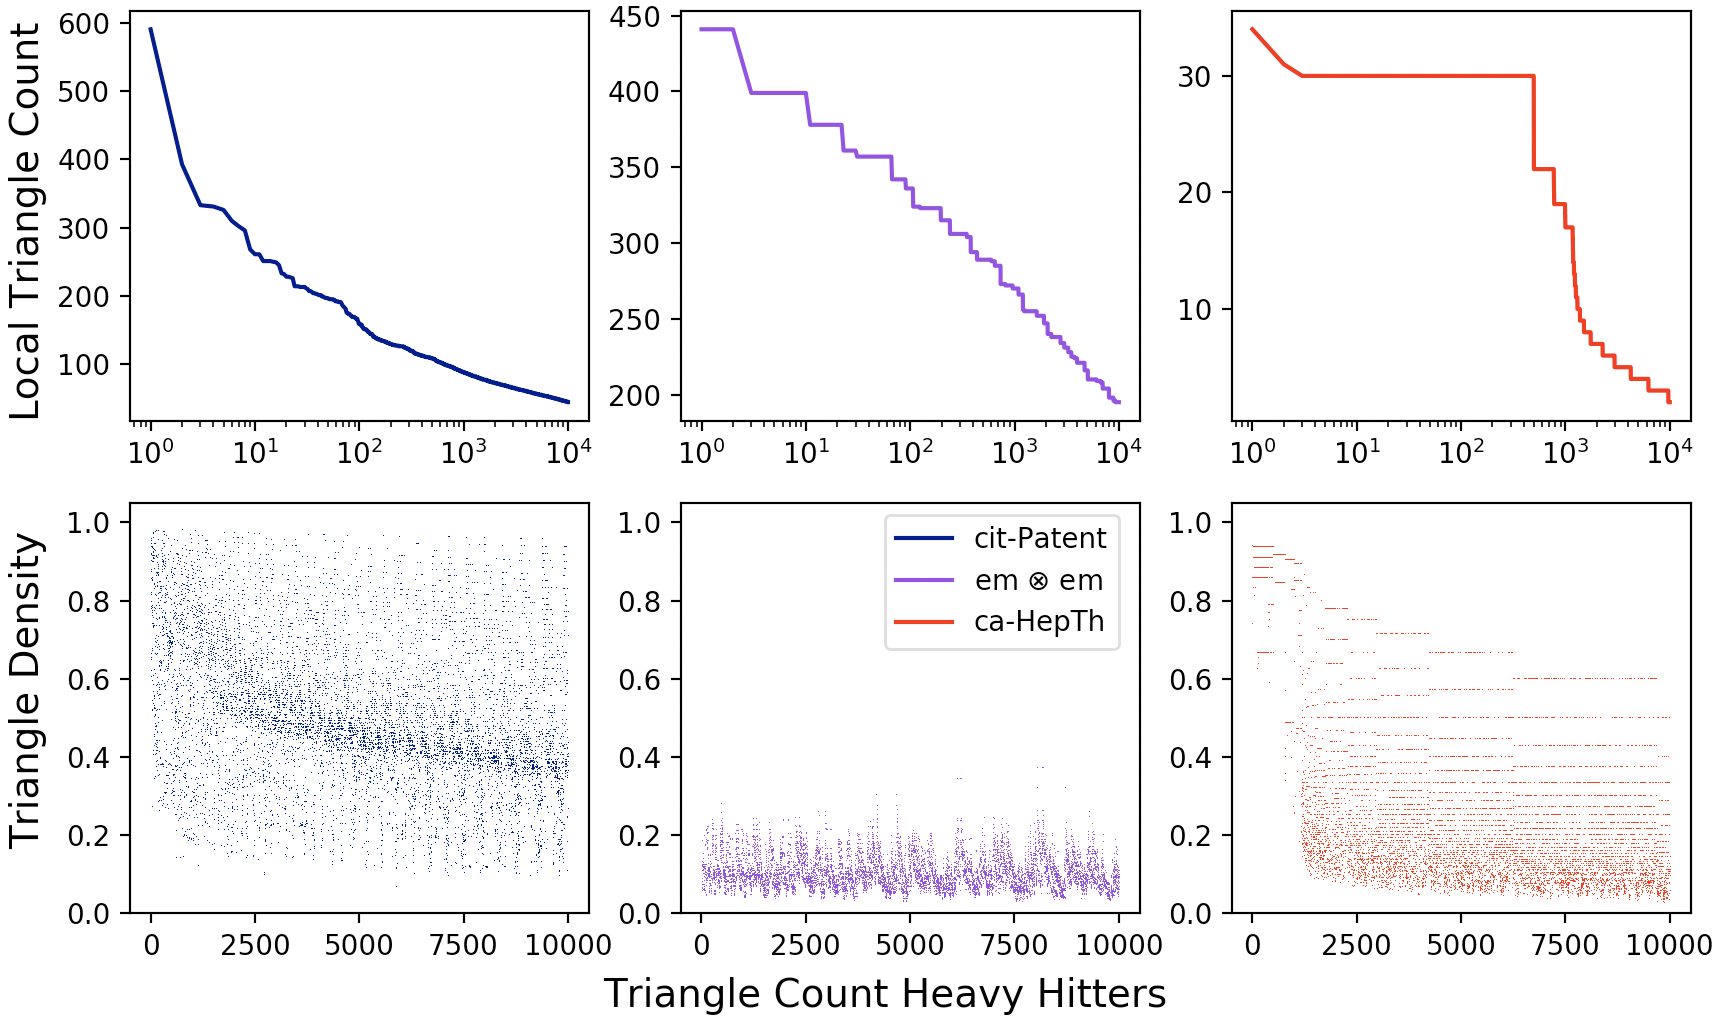
\includegraphics[width=0.9\columnwidth]{hh_comp_3_landscape}}

\begin{block}{}
	\begin{center}
		Low triangle density $\rightarrow$ high variance \\
		Many ties $\rightarrow$ poor recovery
	\end{center}
\end{block}

\end{frame}



%----------------------------------------------------------------------------------------

\begin{frame}
\frametitle{Edge Local Relative Error - Experimental Distributions}

\centerline{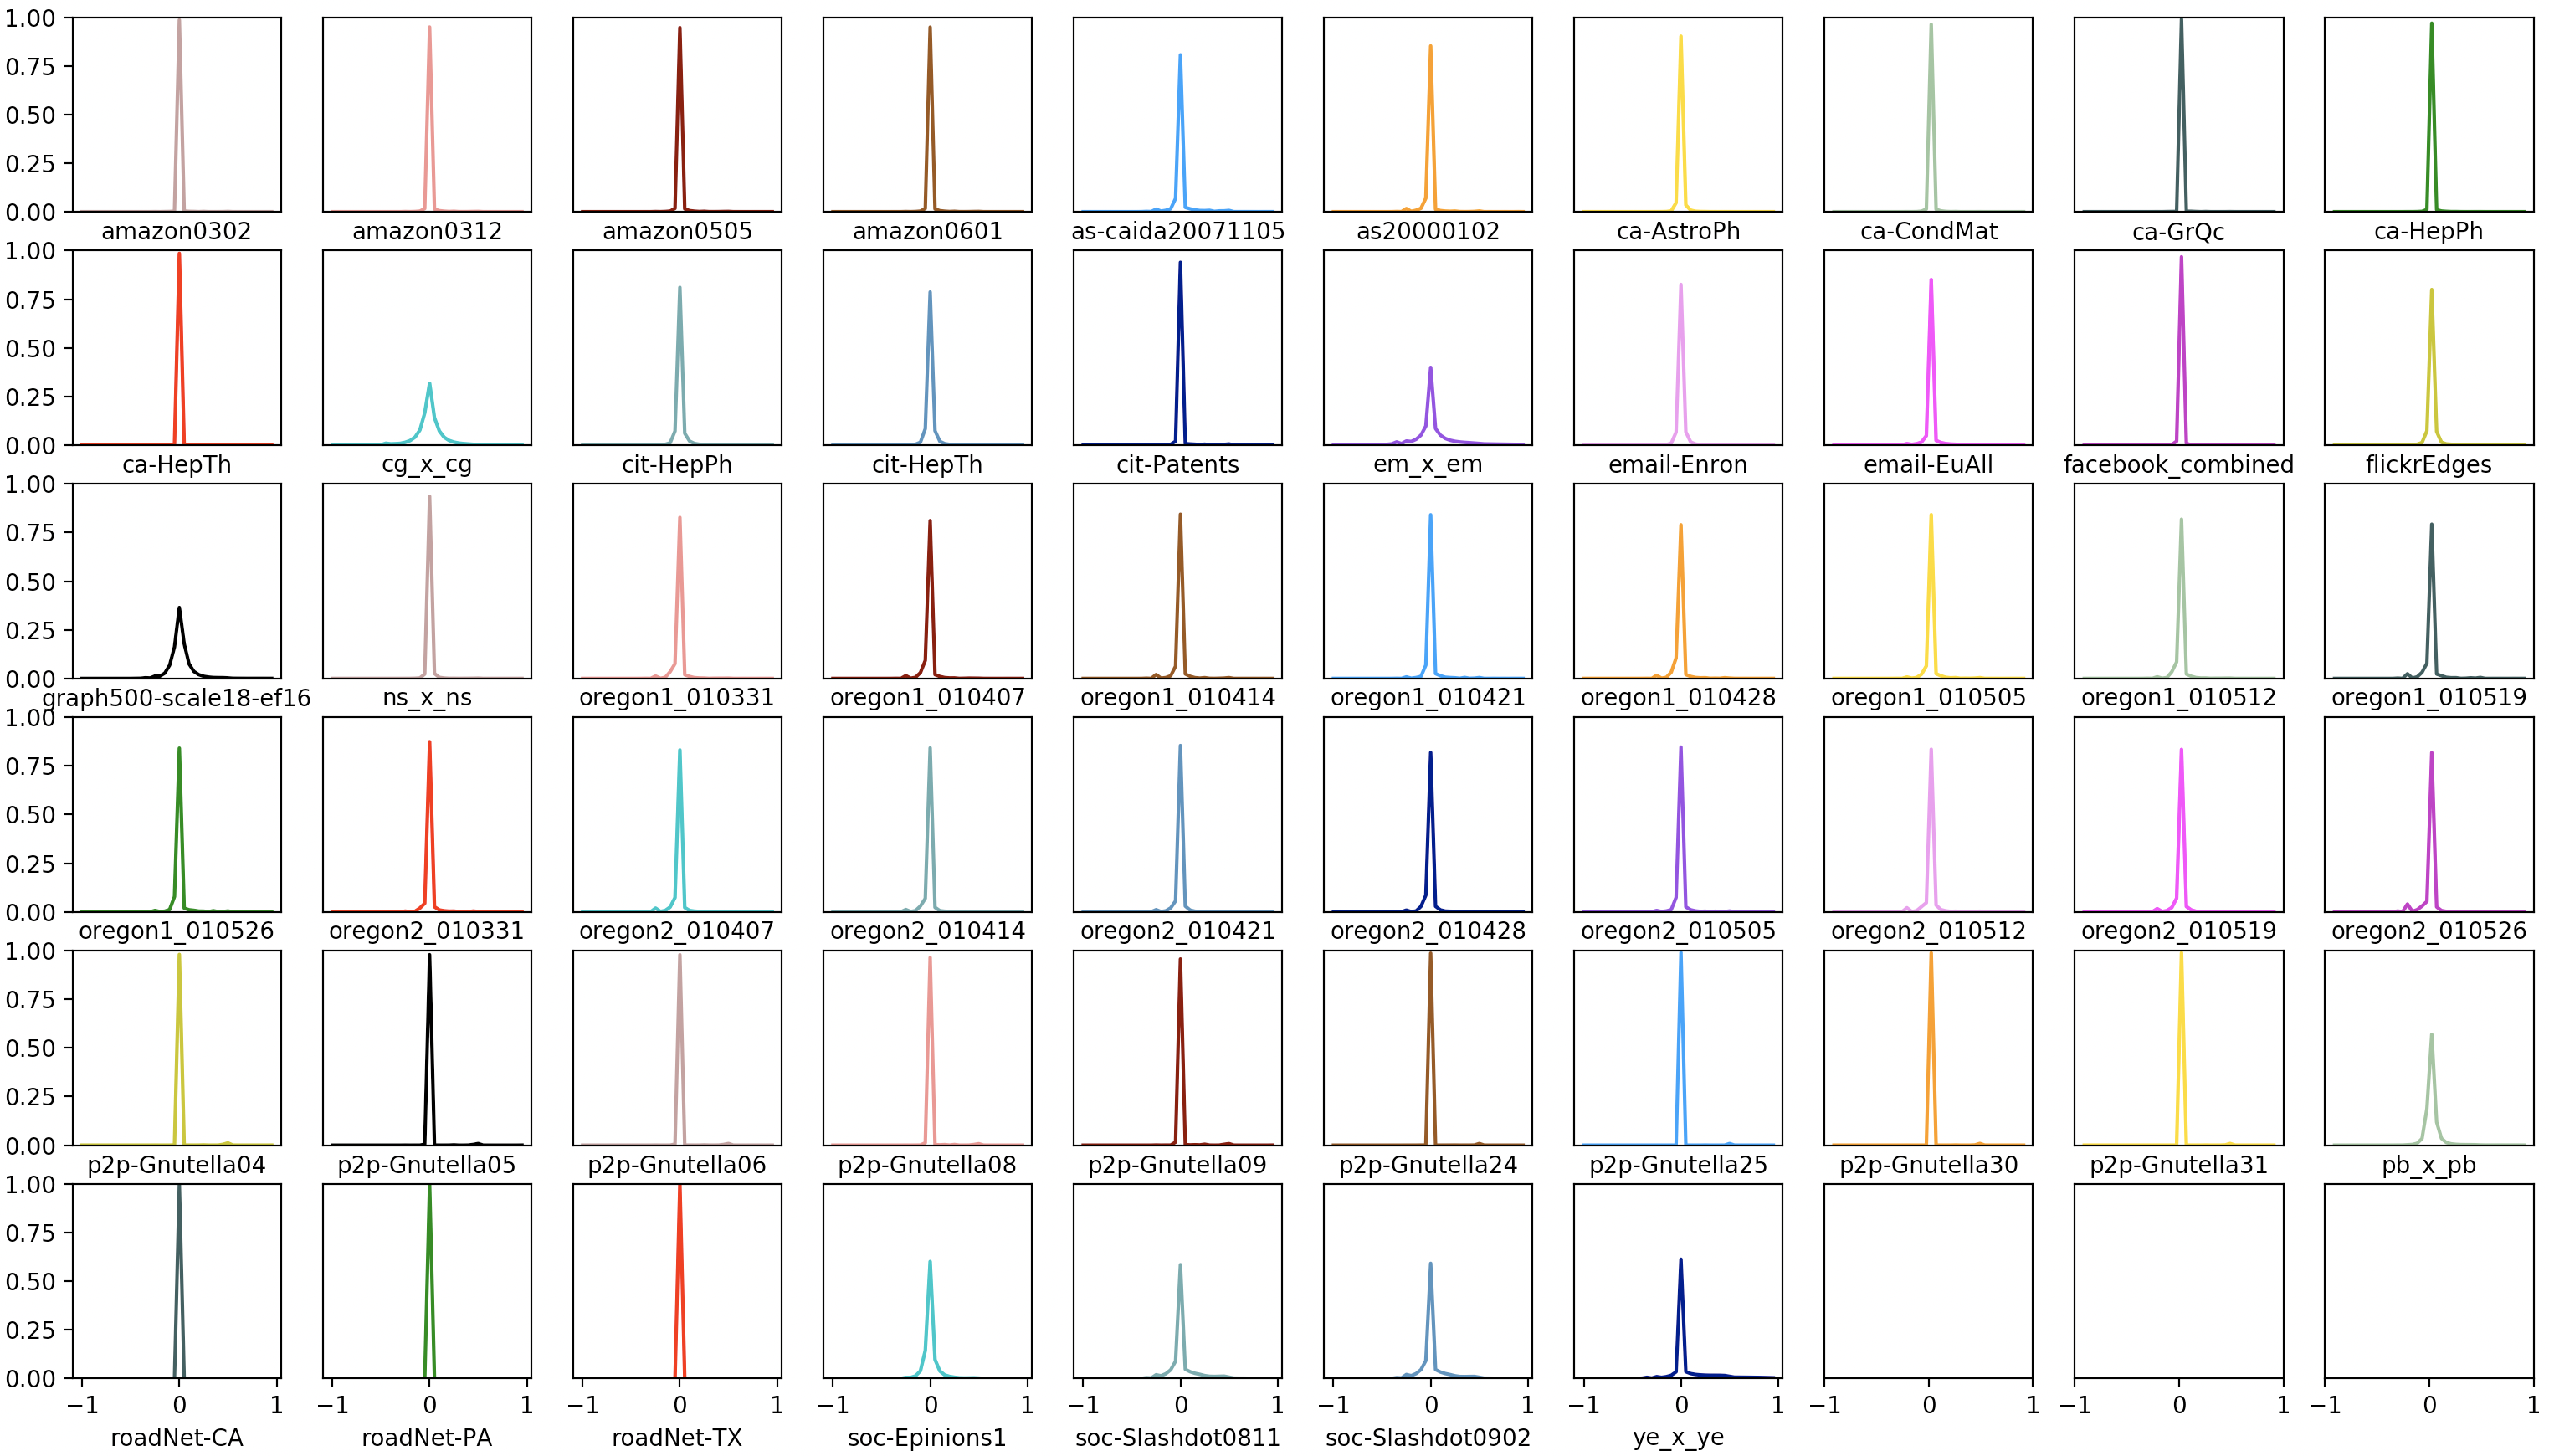
\includegraphics[width=1.0\columnwidth]{distn_edge_total_landscape}}

\begin{block}{}
	\begin{center}
		Good relative error on reasonably sized graphs
	\end{center}
\end{block}

\end{frame}



%----------------------------------------------------------------------------------------

\begin{frame}
\frametitle{Implementation Details}


\textbf{\algoname{DegreeSketch} C++/MPI Library}
\begin{itemize}
	\item Authored by myself
	\item Utilizes \algoname{YGM} for communication
	\item Accumulation and query API for \algoname{DegreeSketch}
	\item Supports sparse and compressed registers
	\item Implementations for edge- and vertex-local triangle count heavy hitter estimation
	\item Supports more exotic queries
	\begin{itemize}
		\item e.g. Intersection of unions
	\end{itemize}
\end{itemize}

\begin{block}{}
	\begin{center}
		\algoname{DegreeSketch} to be open sourced	
	\end{center}
\end{block}

\end{frame}


%----------------------------------------------------------------------------------------
%----------------------------------------------------------------------------------------
\section{Sublinear $\kappa$-Path Centrality}
%----------------------------------------------------------------------------------------
%----------------------------------------------------------------------------------------

\againframe<7>{overview}

\begin{frame}
\frametitle{Motivation: Betweenness Centrality Heavy Hitters}

\textbf{The Problem}:
\begin{itemize}
	\item Computing Betweenness centrality exactly amounts to computing \algoname{AllSourcesAllShortestPaths}
	\begin{itemize}
		\item Expensive $O(mn)$!
	\end{itemize}
\end{itemize}
\textbf{Existing Solutions}:
\begin{itemize}
	\item Approximate via a logarithmic number of \algoname{SingleSourceAllShortestPaths} \cite{green2012fast, bergamini2014approximating, yoshida2014almost, kourtellis2015scalable, riondato2016fast}
	\begin{itemize}
		\item Difficult to distribute
		\item Unclear if possible in $o(m)$ memory
	\end{itemize}
\end{itemize}


\end{frame}



%----------------------------------------------------------------------------------------

\begin{frame}
\frametitle{Approach: Semi-Streaming $\kappa$-Path Centrality}

\textbf{Idea}: ``Come at the problem sideways''
\begin{itemize}
	\item High $\kappa$-path centrality empirically correlates with high betweenness centrality \cite{kourtellis2013identifying}%[KTSIT13]
	\item Algorithm amounts to sampling random simple paths
	\begin{itemize}
		\item Sublinearize by accumulating a fixed number of sketches ahead of time
	\end{itemize}
	\item Sublinear approximation of $\kappa$-path centrality $\rightarrow$ emprical recovery of high betweenness centrality vertices?
\end{itemize}

\begin{dynblock}
% kappa-path centrality
\opaqueblock<1>{
%
$\kappa$-path centrality
\begin{center}
$\mathcal{C}^{\algoname{Path}}_\kappa(x) =  \Pr_{p: |p| \leq \kappa} [x \in p \wedge \text{$p$ a simple path} ]$
\end{center}
%
``simple path'' = non-self-intersecting path
}
\end{dynblock}

\begin{block}{}
	\begin{center}
		Must simulate many history-avoiding random walks
	\end{center}
\end{block}

\end{frame}

%----------------------------------------------------------------------------------------

\begin{frame}
\frametitle{Parallel Random Walk Simulation - Lower Bound}

\begin{block}{Lemma (\algoname{Index} Problem)}
Alice gets $X \in \{0,1\}^n$ and Bob gets $i \in [n]$.
Alice must send $\Omega(n)$ bits for Bob to guess $X_i$ w. p. $>\frac{1}{2}$.
\end{block}

\begin{block}{Theorem 7.2.2}
For $t = O(n^2)$ and $k = O(n^2)$, simulating $k$ $t$-step random walks on a simple undirected graph in the insertion-only model within error $\varepsilon = \frac{1}{3}$ requires $\Omega(n\sqrt{kt})$ space.
\end{block}

\begin{block}{Proof Sketch}
%Depends upon a reduction from the \algoname{Index} problem. 
Alice and Bob agree upon an encoding of $X \in \{0,1\}^{n\sqrt{kt}}$ into a graph partitioned into $\frac{n}{\sqrt{kt}}$ bipartite subgraphs with $2\sqrt{kt}$ vertices.
Bob's index $i \in \left [ n\sqrt{kt} \right ]$ identifies one such subgraph, and $k$ simulated random walks of length $t$ allow probabilistic recovery of $X_i$.
\end{block}




\end{frame}



%----------------------------------------------------------------------------------------

\begin{frame}
\frametitle{Parallel Random Walk Simulation - Lower Bound}


\centerline{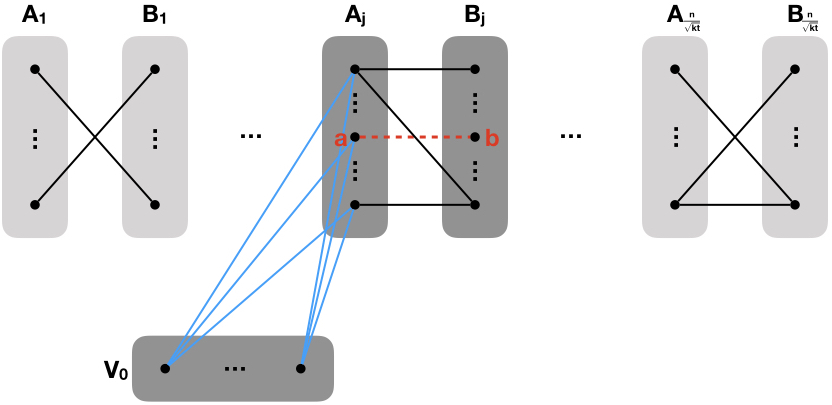
\includegraphics[width=0.9\columnwidth]{lower_bound_proof}}

\begin{block}{}
	\begin{center}
		$i$ indicates $A_j$ and $B_j$, and in particular the edge $ab$.
		Bob adds the blue edges. and simulates $k$ random walks of length $t$ starting in $V_0$. 
		If $ab$ exists, Bob returns $X_i$ with with probability $> \frac{1}{2}, \rightarrow$ solving \algoname{Index}.
	\end{center}
\end{block}




\end{frame}




\begin{frame}
\frametitle{Parallel Random Walk Simulation - Algorithm Outline}

\begin{block}{Lemma 7.1.4 (Reservoir Sampling)}
Given an insert-only stream $\sigma$ consisting of $n$ insertions, there is a procedure that uniformly samples $t \leq \frac{n}{2}$ items with replacement in a single pass using $O(t\log(n/t))$ bits of space. 
\end{block}

\begin{itemize}
%	\item Split $\mathcal{V}$ into big and small sets
%	\begin{itemize}
%		\item $\mathcal{S} = \{x \in \mathcal{V} \mid \mathbf{d}_x \leq c \}$
%		\item $\mathcal{B} = \{x \in \mathcal{V} \mid \mathbf{d}_x > c \}$
%	\end{itemize}
	\item Split $\mathcal{E}$ based upon endpoint degree for a to-be-specified $c$
	\begin{itemize}
		\item $\mathcal{E}_\mathcal{S} = \{(x, y) \in \mathcal{E} \mid \mathbf{d}_y \ \leq c \}$ (important)
		\item $\mathcal{E}_\mathcal{B} = \{(x, y) \in \mathcal{E} \mid \mathbf{d}_y > c \}$ (unimportant)
	\end{itemize}
	\item $|\mathcal{E}_\mathcal{S}| = O(nc)$, so can store in memory if $c$ small enough
	\item In a pass over $\mathcal{G}$, sample $O(c)$ unimportant edges per vertex and build the distributed dictionaries:
	\begin{itemize}
		\item $\mathcal{N}_\mathcal{S}[x] = \{(u, v) \in \mathcal{E}_\mathcal{S} \mid u = x \}$
		\item $\mathcal{N}_\mathcal{B}[x]= \{(u, v) \in \mathcal{E}_\mathcal{B} \mid u = x \wedge \textnormal{$(u, v)$ is sampled} \}$
	\end{itemize}
	\item During each simulation, toss a coin whether to pull from $\mathcal{N}_\mathcal{S}$ or $\mathcal{N}_\mathcal{B}$ at each step
	\begin{itemize}
		\item Simulation \emph{fails} on a vertex if it runs out of unimportant samples
	\end{itemize}
\end{itemize}





\end{frame}


%----------------------------------------------------------------------------------------

\begin{frame}
\frametitle{Parallel Random Walk Simulation - Correctness Outline}


\begin{block}{Lemma 7.2.3}
%Suppose for every $x \in \mathcal{V}$, $\Pr \left [\textnormal{$x$ fails} \mid v_0^{(1)} = x \wedge \left (v_0^{(2)}, \dots, v_0^{(k)} \right ) \right ] \leq \delta$.
%Then for any starting vertex $x \in \mathcal{V}$, $\Pr \left [\textnormal{any vertex fails} \mid v_0^{(1)} = s \wedge \left (v_0^{(2)}, \dots, v_0^{(k)} \right ) \right ] \leq tk\delta$.
Suppose for every $x \in \mathcal{V}$, $\Pr \left [\textnormal{$x$ fails} \mid \textnormal{$x$ a starting vertex} \right ] \leq \delta$.
Then $\Pr \left [\textnormal{any vertex fails} \right ] \leq tk\delta$.
\end{block}

\begin{block}{Lemma 7.2.4}
$\exists c = O\left (\sqrt{kt} \cdot \frac{q}{\log q} \right )$, where $q = 2 + \frac{\log(1/\delta)}{\sqrt{kt}}$ s. t. for all $x \in \mathcal{V}$ 
%
\begin{equation*}
\Pr \left [\textnormal{$x$ fails} \mid \textnormal{$x$ a starting vertex, others drawn from $\mu$} \right ] \leq \delta.\footnote{$\mu$ is the steady state distribution of $\mathcal{G}$}
\end{equation*}
%
%where $x$ does not occur in $\left ( v_0^{(1)}, v_0^{(2)}, \dots, v_0^{(k)} \right )$ more than $\sqrt{k}$ times, 
%for all $x \in \mathcal{V}$.
\end{block}


\begin{block}{Theorem 7.2.5}
Can simulate $k$ $t$-step random walks where sources are drawn with replacement from $\mu$ in a one pass within error $\varepsilon$ using $O \left (n \sqrt{kt} \frac{q}{\log q} \right )$ words of memory, where $q = 2 + \frac{\log(1/\varepsilon)}{\sqrt{kt}}$.
\end{block}


\end{frame}



%----------------------------------------------------------------------------------------
\begin{frame}
\frametitle{Parallel Random Walk Simulation - Extensions in Brief}


\begin{itemize}
	\item Recording and playback of adjacency substreams
	\begin{itemize}
		\item Each processor records $\mathcal{M}[x]$ in faster-than-disc external memory\footnote{e.g. NVRAM} while accumulating $\mathcal{N}_\mathcal{B}[x]$
		%
		\begin{equation*}
			\mathcal{M}[x] = \{ (u, v) \in \mathcal{E}_\mathcal{B} \mid u = x\}
		\end{equation*}
		%
		\item Instead of failing when $\mathcal{N}_\mathcal{B}[x]$ runs out of samples, simply take another pass over $M[x]$
		\begin{itemize}
			\item Partially avoids the steady state distribution heavy hammer		
		\end{itemize}
		\item I/O versus memory tradeoff
		\begin{itemize}
			\item Sublinear storage of graph
			\item Playbacks incur additional I/O on some processors
		\end{itemize}
	\end{itemize}
	\item History-Avoiding Walk Simulation
	\begin{itemize}
		\item Sample via playback, ignoring previous vertices
		\item Permits the sublinear space simulation of simple paths
	\end{itemize}
\end{itemize}





\end{frame}



%----------------------------------------------------------------------------------------

%\begin{frame}
%\frametitle{$\ell_p$ Sampling Sketches}
%
%\begin{dynblock}
%% l2 sampling
%\opaqueblock<1>{
%%
%\textbf{$\ell_p$ sampling sketches} \\
%Sample from frequency vector $\mathbf{f}$ with probability relative to $\ell_p$ norm
%\begin{itemize}
%\item Sample $t_i \sim_R (0,1)$ $\forall i \in [n]$
%\item Rescale updates to $\mathbf{f}_i$ by $1/t_i^{1/p}$
%\item Accumulate \algoname{Tug-of-War}, \algoname{CountSketch}, and $\ell_p$ norm sketches
%\item Use sketches to output \algoname{CountSketch} argmax or FAIL
%\end{itemize}
%%
%}
%\invblock<2->
%
%% Second block
%\opaqueblock<2->[0.4\textwidth]{
%%
%\vspace{-0.5cm}
%%
%%\vspace{-0.5cm}
%%
%\begin{center}
%Outputs $(i,P)$ w.p. $1 - \delta$, where $i \in [n]$ is sampled w.p. $P = (1 \pm \varepsilon)\frac{|v_i|^p}{\|v\|^p_p}$ \cite{monemizadeh20101}
%\end{center}
%}
%%
%
%\end{dynblock}
%
%
%
%\begin{dynblock}
%% rank-k approximation
%\opaqueblock<3>{
%%
%\begin{tabular*}{\textwidth}{l @{\extracolsep{\fill}} r}
%\textbf{Useful results}  & \cite{jowhari2011tight, vu2018data}
%%[CW09]
%\end{tabular*}
%%
%\vspace{-0.5cm}
%%
%\begin{itemize}
%	\item $\ell_0$ sketch requires $\widetilde{O}(\log (1/\delta))$ memory and update time
%	\begin{itemize}
%		\item Useful for unweighted random hops
%	\end{itemize}
%	\item $\ell_1$ sketch requires $\widetilde{O}(\varepsilon^{-1} \log (1/\delta))$ memory and $\widetilde{O}(\log (1/\delta))$ update time
%	\begin{itemize}
%		\item Useful for weighted random hops
%	\end{itemize}
%	\item $s$ parallel $\ell_p$ sketches can be accumulated in time independent of $s$
%\end{itemize}
%}
%\end{dynblock}
%
%
%
%
%\end{frame}

%----------------------------------------------------------------------------------------

%\begin{frame}
%\frametitle{Sublinear Random Walk Simulation}
%
%\textbf{Random Walk Simulation}
%\begin{itemize}
%	\item Sample $t$ vertices $\{v_{1,1}, \dots, v_{t,1}\}$ and: 
%	\begin{itemize}
%		\item Sample $v_{i, j + 1}$ from $\mathcal{A}[v_{i, j}]$
%		\item Communicate $(v_{i, 1}, \dots, v_{i, j + 1})$ to $f(v_{i, j + 1})$
%%		\item When a processor exhausts $s$ sketches for $v$, take another pass over $a_v$ in disk memory 
%	\end{itemize}
%\end{itemize}
%\textbf{Random Simple Path Simulation}
%\begin{itemize}
%	\item Similar to random walks, except:
%	\begin{itemize}
%		\item Do not accumulate sketches ahead of time
%		\item Sample $v_{i, j + 1}$ from $\mathcal{A}[v_{i, j}] \setminus \{v_{i, 1}, \dots, v_{i, j - 1}\}$ 
%		\begin{itemize}
%			\item If $\mathcal{A}[v_{i, j}]$ is not in memory, accumulate a sketch ignoring edges to any of $\{v_{i, 1}, \dots, v_{i, j - 1}\}$
%		\end{itemize}
%		\item Communicate $(v_{i, 1}, \dots, v_{i, j + 1})$ to $f(v_{i, j + 1})$
%	\end{itemize}
%\end{itemize}
%
%\begin{block}{}
%\begin{center}
%Sublinear distributed storage of graph by sketching high degree vertices
%\end{center}
%\end{block}
%
%
%\end{frame}

%----------------------------------------------------------------------------------------



%\begin{frame}
%\frametitle{$\ell_p$ Sampling Graph Sparsification}
%
%
%%\begin{definition}[$\ell_p$-Sampling Sketch]
%%A distribution $\Pi$  on $k \times n$ matrices so that if for any $v \in \mathbb{R}^n$, $S$ drawn from $\Pi$ is such that, given $Sv$, one can produce $i \in [n]$ sampled with probability $(1 \pm \varepsilon)\frac{|v_i|^p}{\|v\|_p}$
%%\end{definition}
%
%\begin{itemize}
%	\item Exploit sketch linearity
%	\begin{itemize}
%		\item Sample $\ell_0$ sampling sketch matrices $S_1, \dots, S_t$, each of which will sketch every column of $B$
%		\item $S_1(B_{:,x})$ returns a sampled neighbor of $x$, say $y$
%		\item $S_2(B_{:,x}) + S_2(B_{:,y}) = S_2(B_{:,x} + B_{:,y})$ returns a sampled neighbor of the supervertex $(x + y)$
%		\item et cetera
%	\end{itemize}
%%	\item {[AGM12-1]} \& [AGM12-2] use this method to solve several problems:
%	\item This method can solve several problems \cite{ahn2012analyzing, ahn2012graph}:
%	\begin{itemize}
%		\item $O(n\polylog n)$ to decide connectivity, k-connectivity, bipartiteness, and to approximate the weight of the MST
%		\item Multipass $\tilde{O}(n^{1+1/\alpha})$ to compute sparsifiers, the exact MST, \textbf{$\alpha$-spanners}, and approximate the maximum weight matching
%	\end{itemize}
%\end{itemize}
%
%\begin{block}{}
%\begin{center}
%We will use similar methods to sample random walks and random simple paths in distributed algorithms
%\end{center}
%\end{block}
%
%\end{frame}

%----------------------------------------------------------------------------------------



%\begin{frame}
%\frametitle{Distributed Accumulation $\ell_p$ Sampling Sketches}
%
%%Recall pseudo-asynchronous communication and let $\mathcal{P}$ and $f$ be as before
%\begin{itemize}
%	\item $P \in \mathcal{P}$ accumulates adjacency set $\mathcal{A}[v]$ for each $v \in \mathcal{V}_P$ %from edge stream
%	\begin{itemize}
%		\item When $\mathcal{A}[v]$ too large, replace it with $s$ $\ell_0$ sampling sketches
%		\item Write current state and all subsequent updates to disk memory % in addition to updating $S_v^{(1)}, \dots, S_v^{(s)}$
%	\end{itemize}
%	\item Queries to $\mathcal{A}[v]$ return a sampled neighbor of $v$
%	\begin{itemize}
%		\item If $\mathcal{A}[v]$ is a set of sketches, one is consumed
%		\begin{itemize}
%			\item If \algoname{Fail}, repeat		
%		\end{itemize}
%		\item Once $\mathcal{A}[v]$ sketches are exhausted, $P$ takes another pass over $v$'s substream in disk memory
%	\end{itemize}
%%	\item {[AGM12-1]} \& [AGM12-2] use this method to solve several problems:
%\end{itemize}
%
%\begin{block}{}
%\begin{center}
%Avoids vertex cuts, exchanging communication for I/O
%\end{center}
%\end{block}
%
%\end{frame}

%----------------------------------------------------------------------------------------

%\begin{frame}
%\frametitle{Sublinear Random Walk and Simple Path Sampling}
%
%\textbf{Random Walk Simulation}
%\begin{itemize}
%	\item Sample $t$ vertices $\{v_{1,1}, \dots, v_{t,1}\}$ and: 
%	\begin{itemize}
%		\item Sample $v_{i, j + 1}$ from $\mathcal{A}[v_{i, j}]$
%		\item Communicate $(v_{i, 1}, \dots, v_{i, j + 1})$ to $f(v_{i, j + 1})$
%%		\item When a processor exhausts $s$ sketches for $v$, take another pass over $a_v$ in disk memory 
%	\end{itemize}
%\end{itemize}
%\textbf{Random Simple Path Simulation}
%\begin{itemize}
%	\item Similar to random walks, except:
%	\begin{itemize}
%		\item Do not accumulate sketches ahead of time
%		\item Sample $v_{i, j + 1}$ from $\mathcal{A}[v_{i, j}] \setminus \{v_{i, 1}, \dots, v_{i, j - 1}\}$ 
%		\begin{itemize}
%			\item If $\mathcal{A}[v_{i, j}]$ is not in memory, accumulate a sketch ignoring edges to any of $\{v_{i, 1}, \dots, v_{i, j - 1}\}$
%		\end{itemize}
%		\item Communicate $(v_{i, 1}, \dots, v_{i, j + 1})$ to $f(v_{i, j + 1})$
%	\end{itemize}
%\end{itemize}
%
%\begin{block}{}
%\begin{center}
%Sublinear distributed storage of graph by sketching high degree vertices
%\end{center}
%\end{block}
%
%
%\end{frame}

%----------------------------------------------------------------------------------------


\begin{frame}
\frametitle{Semi-Streaming $\kappa$-Path Centrality}

\begin{dynblock}
% kappa-path centrality
\opaqueblock<1>{
$\kappa$-Path Centrality Approximation Algorithm (\cite{kourtellis2013identifying}):
\begin{enumerate}
	\item Simulate $T = 2 \kappa^2 n^{1-2\alpha} \ln n$ $(\leq \kappa)$-length simple paths over $\mathcal{G}$
	\begin{itemize}
		\item maintain $count[x]$ for each $x \in \mathcal{V}$
	\end{itemize}
	\item $\widetilde{\mathcal{C}}^{\algoname{Path}}_{\kappa}(x) \gets \frac{count[x]}{2 \kappa n^{-2\alpha} \ln n}$
\end{enumerate}
}
%\invblock<2->

%% Second block
%\opaqueblock<2>[0.6\textwidth]{
%%
%\vspace{-0.5cm}
%%
%\begin{center}
%\end{center}
%}

\end{dynblock}

\begin{block}{Theorem ($\kappa$-Path correctness)}
The serial algorithm runs in $O(\kappa^3 n^{2-2\alpha} \log n)$ time and $\Theta(m)$ space, where accuracy parameter 
$\alpha \in \left [ -\frac{1}{2}, \frac{1}{2} \right ]$.
For each $x \in \mathcal{V}$ it produces estimates $\widetilde{\mathcal{C}}_\kappa^{\algoname{Path}}[x]$ such that 
$\left | \widetilde{\mathcal{C}}_\kappa^{\algoname{Path}}[x] - \mathcal{C}_\kappa^{\algoname{Path}}[x] \right | \leq n^{\frac{1}{2} + \alpha}$ with probability at least $1 - \frac{1}{n^2}$.
\end{block}

\begin{block}{}
	\begin{center}
		Easy application of distributed, semi-streaming history-avoiding random walk simulation
	\end{center}
\end{block}


%\begin{itemize}
%	\item Given $\alpha \in [-1/2,1/2]$, for each $x \in \mathcal{V}$, $\left | \widetilde{\mathcal{C}}^{\algoname{Path}}_{\kappa}(x) -  \mathcal{C}^{\algoname{Path}}_{\kappa}(x) \right | \leq n^{1/2+\alpha}$ w.h.p.
%\end{itemize}

%\begin{dynblock}
%% Sublinear kappa-path centrality
%\opaqueblock<3>{
%Sublinear $\kappa$-Path Centrality Approximation Algorithm
%\begin{enumerate}
%	\item Accumulate $\mathcal{A}$ adjacency query structure
%	\item Sample starting vertices $(v_{1,1}, \dots, v_{T,1})$ and lengths $()$Sketch each column of $B$ (node-edge incidence matrix) in parallel over $\kappa$-rounds ($S_{j,1}, \dots, S_{j,T}$ in round $j$)
%	\item Simulate $T$ simple paths as follows, maintaining $count[x]$ as before:
%	\begin{itemize}
%		\item $x_1 \sim V$,
%		\item $x_2 \sim S_{1,i}(x_1)$
%		\item $x_j \sim S_{j,i} \left ( x_{j-1}\right )$, where $S_{j,i}$ is accumulated ignoring edges between $x_{j-1}$ and any of $x_1, \dots, x_{j-2}$
%	\end{itemize}
%	\item $\widetilde{\textnormal{PC}}(x, \kappa) \gets \frac{count[x]}{2 \kappa n^{-2\alpha} \ln n}$
%\end{enumerate}
%}
%\invblock<4->
%
%% Second block
%\opaqueblock<4>[0.8\textwidth]{
%%
%\vspace{-0.5cm}
%%
%\begin{center}
%$T = 2 \kappa^2 n^{1-2\alpha} \ln n$ is a lot of sketches to store \\
%$\kappa$ might be a large number of passes over input
%\end{center}
%}
%%\end{dynblock}
%\invblock<5->
%
%% Second block
%\opaqueblock<5>[0.6\textwidth]{
%%
%\vspace{-0.5cm}
%%
%\begin{center}
%Can we find a sampling algorithm or variant centrality index that affords a sublinear-space approximation of this form?
%\end{center}
%}
%\end{dynblock}



\end{frame}

	
%----------------------------------------------------------------------------------------


%\begin{frame}
%\frametitle{Sublinear $\kappa$-Path Centrality}
%
%\begin{algorithm}[H]
%\caption{Sublinear $\kappa$-Path Centrality}\label{alg:sublinear_kpath}
%\begin{algorithmic}[1]
%%\State $T \gets 2 \kappa^2 n^{1-2\alpha} \ln n$
%\For {$i \in \{1, \dots, T\}$}
%	\State $p_i \gets$ empty path
%	\State $p_{i,1} \gets$ uniform sample from $\mathcal{V}$
%	\State $l_i \gets$ uniform sample from $\{1, 2, \dots, \kappa \}$
%\EndFor
%\For {$x \in \mathcal{V}$}{$c_x \gets 0$}
%\EndFor
%\ParFor{$j \in \{1, 2, \dots, \kappa - 1 \}$} 
%	\ParFor {$i \in \{1, 2, \dots, T\}$}
%		\If {$j < l_i$}
%			\State $p_{i,j+1} \gets$ sample from $\mathcal{A}[p_{i,j}]$
%			\If {$p_{i,j+1} = \emptyset$}{ discard}
%			\EndIf
%		\ElsIf {$j = l_i$}
%			\State $c_{p_{i,k}} \gets c_{p_{i,k}} + 1$ for $k \in \{1, \dots, j\}$
%		\EndIf
%	\EndParFor
%\EndParFor
%\State \Return $c_x /  2 \kappa n^{-2\alpha} \ln n$ for $x \in V$
%\end{algorithmic}
%\end{algorithm}
%
%
%
%\end{frame}





%----------------------------------------------------------------------------------------


%\begin{frame}
%\frametitle{Sublinear Approximation of Dominant Left Eigenvector}
%
%\begin{dynblock}
%% Eigencentrality
%\opaqueblock<1>{
%Eigencentrality
%\begin{itemize}
%	\item Let $A = Q \Lambda Q^{-1}$ be the eigendecomposition of $G$'s adjacency matrix
%	\item $\textnormal{EC}(x) = Q_{1,x}$
%\end{itemize}
%}
%\invblock<2->
%
%% Second block
%\opaqueblock<2>[0.6\textwidth]{
%%
%\vspace{-0.5cm}
%%
%\begin{center}
%Variants: Katz's index, \algoname{PageRank}, \algoname{HITS}, \algoname{SALSA}, \dots
%\end{center}
%}
%\end{dynblock}
%
%
%\begin{dynblock}
%% Question
%\opaqueblock<3->{
%\textbf{Q}: How to sublinearly approximate $Q_{1,:}$?
%%
%\begin{itemize}
%	\item For general square matrices?
%	\item For adjacency matrices of graphs?
%	\item For adjacency matrices of a class of graphs?
%\end{itemize}
%}
%\end{dynblock}
%
%
%
%\begin{dynblock}
%% Answer
%\opaqueblock<4->{
%%
%\textbf{A:} Use low-rank approximations \cite{andoni2013eigenvalues}%[AN13]
%%
%\begin{itemize}
%	\item e.g. sketched SVD-like approximations \cite{sarlos2006improved, clarkson2009numerical, clarkson2017low} or CUR approximations \cite{boutsidis2017optimal}%[DKM06], [DMM08], [BW14] 
%%	\item e.g. sketched SVD-like approximations [S06], [CW09], [CW13] or CUR approximations [DKM06], [DMM08], [BW14] 
%	\item Use factored output $\tilde{A}_k = \tilde{U} \tilde{\Sigma} \tilde{V}^T$ to approximate eigendecomposition
%\end{itemize}
%}
%
%\invblock<5->
%
%% Second block
%\opaqueblock<5>[0.85\textwidth]{
%%
%\vspace{-0.5cm}
%%
%\begin{center}
% Such $\tilde{A}_k$ satisfies $\|A-\tilde{A}_k\|_F \leq (1+\varepsilon) \| A - A_k \|_F$ w.h.p. \\
% There is \textbf{no} guarantee that the approximate singular vectors or that so-constructed eigenvectors will be close to those of $A$
%\end{center}
%}
%
%\end{dynblock}
%
%
%\end{frame}



%----------------------------------------------------------------------------------------


%\begin{frame}
%\frametitle{Sublinear Approximation of Dominant Left Eigenvector}
%
%
%\begin{dynblock}
%% Question
%\opaqueblock<1->{
%\textbf{Q}: So what do we do?
%}
%\end{dynblock}
%
%\begin{dynblock}
%% Answer 1
%\opaqueblock<2->{
%\textbf{A1}: Try it!
%\begin{itemize}
%	\item Low-rank SVD-like approximations still have a lot of $A$'s structure
%	\item May prove empirically useful
%	\item Ennables use of bicriteria solution $AR(SAR)^+SA$ from \cite{clarkson2009numerical}%[CW09]
%	\begin{itemize}
%		\item \textbf{much} faster than true rank-$k$ approximation
%	\end{itemize}
%\end{itemize}
%}
%\end{dynblock}
%
%
%\begin{dynblock}
%% Answer 1
%\opaqueblock<3->{
%\textbf{A2}: Novel algorithms!
%\begin{itemize}
%	\item Bounded-error solution desirable
%	\item Possibly take advantage of structure, like \algoname{HITS} approximation
%	\begin{itemize}
%		\item Limited to graphs, specific classes of graphs, tree width, \dots
%	\end{itemize}
%\end{itemize}
%}
%\end{dynblock}
%
%
%
%\end{frame}



%----------------------------------------------------------------------------------------


%\begin{frame}
%\frametitle{Robustness of Sketches?}
%
%
%\begin{dynblock}
%% Question
%\opaqueblock<1->{
%\textbf{Q}: What happens if there are noisy or malicious updates?
%\begin{itemize}
%	\item Input $v = v^{(g)} + v^{(b)}$
%	\item $S(v) = S(v^{(g)}) + S(v^{(b)})$
%	\item Possible to recover $S(v^{(g)})$ from $S(v)$?
%	\item Overlap during distributed computation?
%\end{itemize}
%}
%\end{dynblock}
%
%
%\begin{dynblock}
%% Answer
%\opaqueblock<2->{
%\textbf{A}: I have no idea
%\begin{itemize}
%	\item I just started thinking about this problem last week
%	\item \cite{hadjieleftheriou2005robust} addresses robustness of distributed sketches
%	\item \cite{hardt2013robust} discusses robustness of \emph{adaptive} streams
%%	\item {[HBK05]} addresses robustness of distributed sketches
%%	\item{[HW13]} discusses robustness of \emph{adaptive} streams
%	\item Certainly important to address for practical implementation
%\end{itemize}
%}
%\end{dynblock}
%
%
%\end{frame}



%----------------------------------------------------------------------------------------


%\begin{frame}
%\frametitle{Implementation and Empirical Evaluation}
%
%\begin{itemize}
%	\item Research goals require empirical evaluation
%	\begin{itemize}
%		\item Disciplined code implementation
%		\item Experiments on real and synthetic data
%		\item Display value of approach to applied community
%	\end{itemize}
%	\item Requires software!
%	\begin{itemize}
%		\item ``Leave-behind'' scientific contribution
%		\item Leverage existing tools
%		\begin{itemize}
%			\item \textbf{libskylark}: Python/C++ sketch library
%			\item \textbf{libelemental}: Python/C++ distributed matrix library
%		\end{itemize}
%	\end{itemize}
%\end{itemize}
%
%
%
%\end{frame}



%----------------------------------------------------------------------------------------


\begin{frame}
\frametitle{Summary of Results}

\begin{itemize}
	\item The Goal: distributed semi-streaming approximations of centrality indices
	\item Engineering Results
	\begin{itemize}
		\item \algoname{YGM}: Pseudo-Asynchronous 	Communication Handler
	\end{itemize}
	\item Algorithmic Results
	\begin{itemize}
		\item A streaming degree centrality approximation and heavy hitter recovery algorithms
		\item A O(1)-pass semi-streaming closeness centrality approximation algorithm
		\item 2-pass distributed semi-streaming local neighborhood and triangle count estimation algorithms using \algoname{DegreeSketch}
		\item Distributed semi-streaming random walk simulation algorithm
		\item Distributed sublinear semi-streaming $\kappa$-path centrality estimation algorithm
	\end{itemize}
	\item Future Work
	\begin{itemize}
		\item Applications for $\algoname{DegreeSketch}$
		\item Semi-streaming random walk with playback implementation
	\end{itemize}
\end{itemize}

\end{frame}


%----------------------------------------------------------------------------------------

\begin{frame}
\frametitle{Dartmouth Publications}

{\tiny
\begin{enumerate}
\item \textbf{Benjamin W. Priest} and George Cybenko.
	Efficient inference of hidden Markov models from large observation sequences.
	In \emph{Proceedings of the 2016 SPIE Defense + Security Conference}, 
	SPIE D$\! + \!$S.
	2016.

\item \textbf{Benjamin W. Priest} and George Cybenko.
	Approximating centrality in evolving graphs: toward sublinearity.
	In \emph{Proceedings of the 2017 SPIE Defense + Security Conference}, 
	SPIE D$\! + \!$S.
	2017.

\item Luan Hoy Pham, Massimiliano Albanese, and \textbf{Benjamin W. Priest}.
	A quantitative framework to model advanced persistent threats.
	In \emph{Proceedings of the 15th International Conference on Security and Cryptography}, 
	SECRYPT. 
	2018.
	\textbf{[Best Paper Award]}
	
\item \textbf{Benjamin W. Priest}, Roger Pearce, and Geoffrey Sanders.
	Estimating edge-local triangle count heavy hitters in edge-linear time and almost-vertex-linear space.
	In \emph{Proceedings of the IEEE High Performance Extreme Computing Conference}, 
	HPEC. 
	2018.
	
\item \textbf{Bejamin W. Priest}, George Cybenko, Satinder Singh, Massimiliano Albanese and Peng Liu.
	Online and Scalable Adaptive Cyber Defense. 
	In:
	Michael Wellman~(Ed.), \emph{Adversarial and Uncertain Reasoning in Adaptive Cyber-Defense}, ch.
	11, pp. xxx--xxx. 2019.
	\textbf{[In Press]}.

\item \textbf{Benjamin W. Priest}, Trevor Steil, Roger Pearce, and Geoffrey Sanders.
	You've {G}ot {M}ail: Building missing asynchronous communication primitives.
	In:
	GraML Workshop at the 2019 IEEE International Symposium on Parallel and Distributed Processing,
	IPDPS.
	2019.
	\textbf{[To Be Submitted]}.

\item Trevor Steil, \textbf{Benjamin W. Priest}, Roger Pearce, Keita Iwabuchi, Timothy LaFond, and Geoff Sanders. 
	Massive-scale graph generation with ground truth: Triangles, centrality, and communities.
	GraPL Workshop at the 2019 IEEE International Symposium on Parallel and Distributed Processing,
	IPDPS.
	2019.
	\textbf{[To Be Submitted]}.
	
\item \textbf{Benjamin W. Priest}, Roger Pearce, and Geoffrey Sanders.
	DegreeSketch: Distributed cardinality sketches on graphs with applications.
	\textbf{[In Preparation]}.

\item \textbf{Benjamin W. Priest}.
	Efficient distributed and semi-streaming simulation of random walks.
	\textbf{[In Preparation]}.
\end{enumerate}
}

\end{frame}


\begin{frame}

\begin{center}
{\Huge Questions?}
\end{center}

\end{frame}


%----------------------------------------------------------------------------------------
\bibliography{../../eed1a7a966f874f4aa88bc8e943e71ce/bibliography.bib} 
\bibliographystyle{alpha} 
%\nobibliography{sketching-centrality} 
%\bibliographystyle{alpha}


\end{document} 